% Options for packages loaded elsewhere
\PassOptionsToPackage{unicode}{hyperref}
\PassOptionsToPackage{hyphens}{url}
\PassOptionsToPackage{dvipsnames,svgnames,x11names}{xcolor}
%
\documentclass[
  number]{elsarticle}

\usepackage{amsmath,amssymb}
\usepackage{iftex}
\ifPDFTeX
  \usepackage[T1]{fontenc}
  \usepackage[utf8]{inputenc}
  \usepackage{textcomp} % provide euro and other symbols
\else % if luatex or xetex
  \usepackage{unicode-math}
  \defaultfontfeatures{Scale=MatchLowercase}
  \defaultfontfeatures[\rmfamily]{Ligatures=TeX,Scale=1}
\fi
\usepackage{lmodern}
\ifPDFTeX\else  
    % xetex/luatex font selection
\fi
% Use upquote if available, for straight quotes in verbatim environments
\IfFileExists{upquote.sty}{\usepackage{upquote}}{}
\IfFileExists{microtype.sty}{% use microtype if available
  \usepackage[]{microtype}
  \UseMicrotypeSet[protrusion]{basicmath} % disable protrusion for tt fonts
}{}
\makeatletter
\@ifundefined{KOMAClassName}{% if non-KOMA class
  \IfFileExists{parskip.sty}{%
    \usepackage{parskip}
  }{% else
    \setlength{\parindent}{0pt}
    \setlength{\parskip}{6pt plus 2pt minus 1pt}}
}{% if KOMA class
  \KOMAoptions{parskip=half}}
\makeatother
\usepackage{xcolor}
\setlength{\emergencystretch}{3em} % prevent overfull lines
\setcounter{secnumdepth}{5}
% Make \paragraph and \subparagraph free-standing
\ifx\paragraph\undefined\else
  \let\oldparagraph\paragraph
  \renewcommand{\paragraph}[1]{\oldparagraph{#1}\mbox{}}
\fi
\ifx\subparagraph\undefined\else
  \let\oldsubparagraph\subparagraph
  \renewcommand{\subparagraph}[1]{\oldsubparagraph{#1}\mbox{}}
\fi


\providecommand{\tightlist}{%
  \setlength{\itemsep}{0pt}\setlength{\parskip}{0pt}}\usepackage{longtable,booktabs,array}
\usepackage{calc} % for calculating minipage widths
% Correct order of tables after \paragraph or \subparagraph
\usepackage{etoolbox}
\makeatletter
\patchcmd\longtable{\par}{\if@noskipsec\mbox{}\fi\par}{}{}
\makeatother
% Allow footnotes in longtable head/foot
\IfFileExists{footnotehyper.sty}{\usepackage{footnotehyper}}{\usepackage{footnote}}
\makesavenoteenv{longtable}
\usepackage{graphicx}
\makeatletter
\def\maxwidth{\ifdim\Gin@nat@width>\linewidth\linewidth\else\Gin@nat@width\fi}
\def\maxheight{\ifdim\Gin@nat@height>\textheight\textheight\else\Gin@nat@height\fi}
\makeatother
% Scale images if necessary, so that they will not overflow the page
% margins by default, and it is still possible to overwrite the defaults
% using explicit options in \includegraphics[width, height, ...]{}
\setkeys{Gin}{width=\maxwidth,height=\maxheight,keepaspectratio}
% Set default figure placement to htbp
\makeatletter
\def\fps@figure{htbp}
\makeatother

\makeatletter
\@ifpackageloaded{caption}{}{\usepackage{caption}}
\AtBeginDocument{%
\ifdefined\contentsname
  \renewcommand*\contentsname{Table of contents}
\else
  \newcommand\contentsname{Table of contents}
\fi
\ifdefined\listfigurename
  \renewcommand*\listfigurename{List of Figures}
\else
  \newcommand\listfigurename{List of Figures}
\fi
\ifdefined\listtablename
  \renewcommand*\listtablename{List of Tables}
\else
  \newcommand\listtablename{List of Tables}
\fi
\ifdefined\figurename
  \renewcommand*\figurename{Figure}
\else
  \newcommand\figurename{Figure}
\fi
\ifdefined\tablename
  \renewcommand*\tablename{Table}
\else
  \newcommand\tablename{Table}
\fi
}
\@ifpackageloaded{float}{}{\usepackage{float}}
\floatstyle{ruled}
\@ifundefined{c@chapter}{\newfloat{codelisting}{h}{lop}}{\newfloat{codelisting}{h}{lop}[chapter]}
\floatname{codelisting}{Listing}
\newcommand*\listoflistings{\listof{codelisting}{List of Listings}}
\makeatother
\makeatletter
\makeatother
\makeatletter
\@ifpackageloaded{caption}{}{\usepackage{caption}}
\@ifpackageloaded{subcaption}{}{\usepackage{subcaption}}
\makeatother
\ifLuaTeX
  \usepackage{selnolig}  % disable illegal ligatures
\fi
\usepackage[]{natbib}
\bibliographystyle{elsarticle-num}
\usepackage{bookmark}

\IfFileExists{xurl.sty}{\usepackage{xurl}}{} % add URL line breaks if available
\urlstyle{same} % disable monospaced font for URLs
\hypersetup{
  pdftitle={Draft -- Discriminating Seagrasses From Green Macroalgae in European Intertidal areas using high resolution multispectral drone imagery -- Draft},
  pdfauthor={Simon Oiry; Bede Ffinian Rowe Davies; Ana I. Sousa; Philippe Rosa; Maria Laura Zoffoli; Guillaume Brunier; Pierre Gernez; Laurent Barillé},
  pdfkeywords={Drone, Remote Sensing, Seagrass, Coastal
Ecosystems, Neural Network},
  colorlinks=true,
  linkcolor={blue},
  filecolor={Maroon},
  citecolor={Blue},
  urlcolor={Blue},
  pdfcreator={LaTeX via pandoc}}

\setlength{\parindent}{6pt}
\begin{document}

\begin{frontmatter}
\title{Draft -- Discriminating Seagrasses From Green Macroalgae in
European Intertidal areas using high resolution multispectral drone
imagery -- Draft}
\author[1]{Simon Oiry%
\corref{cor1}%
}
 \ead{oirysimon@gmail.com} 
\author[1]{Bede Ffinian Rowe Davies%
%
}

\author[2]{Ana I. Sousa%
%
}

\author[1]{Philippe Rosa%
%
}

\author[3]{Maria Laura Zoffoli%
%
}

\author[4]{Guillaume Brunier%
%
}

\author[1]{Pierre Gernez%
%
}

\author[1]{Laurent Barillé%
%
}


\affiliation[1]{organization={Institut des Substances et Organismes de
la Mer, ISOMer, Nantes Université, UR 2160, F-44000 Nantes,
France},,postcodesep={}}
\affiliation[2]{organization={ECOMARE - Laboratory for Innovation and
Sustainability of Marine Biological Resources, CESAM -- Centre for
Environmental and Marine Studies, Department of Biology, University of
Aveiro, Campus Universitário de Santiago, 3810-193 Aveiro,
Portugal},,postcodesep={}}
\affiliation[3]{organization={Consiglio Nazionale delle Ricerche,
Istituto di Scienze Marine (CNR-ISMAR), 00133 Rome,
Italy},,postcodesep={}}
\affiliation[4]{organization={BRGM French Geological Survey, Cayenne
97300, French Guiana},,postcodesep={}}

\cortext[cor1]{Corresponding author}








        
\begin{abstract}
Coastal areas support seagrass meadows, which offer crucial ecosystem
services including erosion control and carbon sequestration. However,
these areas are increasingly impacted by human activities, leading to
habitat fragmentation and seagrass decline. In situ surveys,
traditionally performed to monitor these ecosystems face limitations on
temporal and spatial coverage, particularly in intertidal zones,
prompting the addition of satellite data within monitoring programs.
Yet, satellite remote sensing struggles with spatial and spectral
resolution, making it difficult to discriminate seagrass from other
macrophytes in highly heterogenous meadows. Drone (unmanned aerial
vehicles -- UAV) images at a very high spatial resolution offer a
promising solution to address challenges related to spatial
heterogeneity and intrapixel mixture. This study focuses on using drone
acquisitions with a ten spectral band sensor mirroring those of
Sentinel-2, for mapping intertidal macrophytes and effectively
discriminating between seagrass and green macroalgae. Nine drone flights
were conducted at two different altitudes (12 m and 120 m) across
heterogeneous intertidal European habitats in France and Portugal. Low
altitude flights were used to train a Deep Learning classifier based on
Neural Networks to discrimintate among five taxonomic classes of
intertidal vegetation: Magnoliopsida (Seagrass), Chlorophyceae (Green
macroalgae), Phaeophyceae (Brown algae), Rhodophyceae (Red macroalgae)
and benthic Bacillariophyceae (Diatoms). Classification of drone imagery
resulted in an overall accuracy of 94\% across all the sites and images,
covering a total area of 467 000 m². The model exhibited an accuracy of
96.4\% in identifying seagrass. Importantly, seagrass and green algae
can be discriminated, although they share the same pigment composition.
As the algorithm was developed for a multispectral camera with ten
spectral bands in the visible and near-infrared, it could be adapted to
the Multi-Spectral Instrument (MSI) onboard Sentinel-2 thus offering
promising perspectives for satellite remote sensing of intertidal
biodiversity over lager scales.
\end{abstract}





\begin{keyword}
    Drone \sep Remote Sensing \sep Seagrass \sep Coastal
Ecosystems \sep 
    Neural Network
\end{keyword}
\end{frontmatter}
    
\section{Introduction}\label{introduction}

Coastal areas are vital hotspots for marine biodiversity, with
intertidal seagrass meadows playing a crucial role at the interface
between the land and oceans \citep{unsworth2022}. Seagrass meadows
provide a myriad of ecosystem services to humanity, including carbon
sequestration, oxygen production, protection against sea-level rise and
coastline erosion, and mitigation of eutrophication \citetext{\citealp[
]{unsworth2022}; \citealp{sousa2019blue}}. They serve as vital habitats
for a diverse array of marine and terrestrial species, providing living,
breeding, and feeding grounds \citetext{\citealp[
]{gardner2018}; \citealp[ ]{Zoffoli2022}; \citealp{jankowska2019}}. Due
to the concentration of human activities in coastal zones, seagrass
meadows are directly exposed to and impacted by anthropogenic pressures.
Global regression and fragmentation of seagrass meadows are currently
observed due to climate change, diseases, urbanization, land
reclamation, dredging, competition with alien species, and reduction in
water quality \citetext{\citealp[ ]{nguyen2021}; \citealp[
]{soissons2018}; \citealp[ ]{orth2006}; \citealp[ ]{lin2018}; \citealp[
]{duffy2019}; \citealp[ ]{rasheed2011long}; \citealp[
]{chefaoui2018dramatic}; \citealp{sousa2019blue}}. Both habitat
fragmentation and reduction, in turn, can severely compromise the
effectiveness of ecosystem services provided by seagrass meadows. While
improvements in water quality and hydrodynamics have been recently
reported in Europe, allowing an overall recovery of seagrass ecosystems
at local and European scales, many coastal waters worldwide are still
subjected to strong eutrophication processes \citetext{\citealp[
]{deSantos2019}; \citealp[ ]{Zoffoli2021}; \citealp{sousa2019blue}}.
Coastal eutrophication has been associated to excessive accumulation of
green macroalgae, so-called green tides \citep{devlin2023nutrients}.
Green tides produce shade and suffocation over seagrass individuals,
thus threatening the health of seagrass ecosystems \citep{wang2022}.

The importance of seagrass meadows and the variety of ecosystem services
they provide have led to the enhancement of both global and regional
programs to monitor Essential Oceanic Variable (EOVs) such as seagrass
composition \citep{Miloslavich2018}, as well as Essential Biodiversity
Variable (EBVs) such as seagrass taxonomic diversity, species
distribution, population abundance, and phenology \citep{Pereira2013}.
Traditionally, indicators of seagrass status have been quantified using
\emph{in situ} measurements. However, the acquisition of these
measurements in intertidal zones is notoriously challenging. Intertidal
seagrass meadows are only exposed during low tide and can be situated in
difficult-to-reach mudflats, potentially leading to inaccurate and
limited estimations with conventional sampling techniques
\citep{nijland2019}. Satellite observations have been proven effective
in complementing \emph{in situ} sampling, allowing for the near
real-time and consistent retrieval of seagrass EOVs and EBVs over
extensive meadows. \citetext{\citealp[ ]{Zoffoli2021}; \citealp[
]{xu2021}; \citealp[ ]{Traganos2018}; \citealp{coffer2023}}

While satellite remote sensing (RS) provides temporally consistent
observations over large spatial scales, its utilization over intertidal
areas is limited by several constraints. Satellite missions with a high
temporal resolution (e.g.~daily MODIS observation) are limited by a too
coarse spatial resolution (\textgreater100 m) to accurately map patchy
seagrass meadows. Missions with a high spatial resolution such as
Sentinel-2 (10 m) or Landsat8/9 (30 m) can be limited by low spectral
resolution. The limited number of spectral bands challenges accurate
discrimination of seagrass from other co-existing macrophytes. In
particular Chlorophyceae (green algae) and marine Magnoliopsida
(seagrass) share the same pigment composition \citetext{\citealp[
]{ralph2002}; \citealp{Douay2022}}. Therefore, to someone not
specialized in the field, their spectral signatures may appear to be
alike \citetext{\citealp[ ]{Davies2023}; \citealp{bannari2022}}.
Recently, using advanced machine-learning algorithms trained with a
large hyperspectral library of more than 300 field reflectance spectra,
\citep{Davies2023} demonstrated that it was possible to discriminate
Magnoliopsida from Chlorophyceae using radiometric data acquired at
Sentinel-2 's spectral resolution. However the application of this
approach to satellite RS remains to be validated. Moreover patches of
green algae can develop at small spatial scales that are not observable
using non-commercial satellite imagery \citep{tuya2013}, especially
during the initial stage of a green tide.

Drones (Unmanned Aerial Vehicles -- UAVs) can potentially fill the data
gaps left by satellite RS and \emph{in situ} measurements, due to their
ability to provide spatially-explicit observations at very high spatial
resolutions (pixel size from mm to cm) while capturing data at
multi-spectral resolution \citetext{\citealp[
]{fairley2022drone}; \citealp{oh2017use}}. The versatility of drones
allows for their application across a diverse thematic range , from
coastal zone management \citetext{\citealp[ ]{adade2021}; \citealp[
]{casella2020}; \citealp{angnuureng2022}} to mapping species
distribution \citetext{\citealp[ ]{joyce2023}; \citealp[
]{tallam2023}; \citealp[ ]{Roca2022}; \citealp[ ]{Roman2021}; \citealp[
]{Brunier2022Topographic}; \citealp{sousa2019blue}}. However, when
applied to coastal habitat mapping, most case studies were previously
limited to a single flight, restricting the generalizability of their
application over wider geographical scales \citetext{\citealp[
]{Roman2021}; \citealp[ ]{collin2019improving}; \citealp[
]{rossiter2020uav}; \citealp{Brunier2022Topographic}}. The present study
aimed at analyzing the potential of multispectral drone RS to map
intertidal macrophytes over a diverse biogeographical range, with a
particular focus on discriminating Magnoliopsida and Chlorophyceae
(Seagrass and Green Algae, respectively). Ten drone flights were
performed over soft-bottom intertidal areas along the Atlantic
coastlines of two European countries (France and Portugal), covering a
wide range of habitats, from monospecific seagrass meadows to meadows
mixed with green, or red macroalgae. A deep learning algorithm was
trained and validated for macrophyte discrimination, emphasizing
applicability across diverse sites without a loss of prediction
accuracy.

\section{Material \& Methods}\label{material-methods}

\subsection{Study sites}\label{study-sites}

Seven study sites distributed between France and Portugal were selected
for their relatively extensive intertidal seagrass beds. Two sites were
located in the Gulf of Morbihan (Figure~\ref{fig-map} A), France
(47.5791°N, 2.8018°W). This gulf covers an area of 115 km² and is only
connected to the sea through a 900 m wide channel. A total of 53 small
islands are scattered across the gulf leading to 250 km of shorelines.
Patchy seagrass meadows can be found on many of these islands. One of
the sites within the gulf was on one its islands (Arz) and the other was
located further south on a mainland beach area (Duer). Two other sites
were located in Bourgneuf Bay, France (46.9849°N, 2.1488°W). This is a
340 km² semi-enclosed macrotidal bay, protected from waves by
Noirmoutier Island. Bourgneuf bay hosts a large intertidal seagrass
meadow of about 6 km² \citep{ZOFFOLI2020112020}. Within this meadow, the
sites observed by drones (L'Epine and Barbatre, Figure~\ref{fig-map} B)
contained monospecific beds of \emph{Nanozostera noltei} (dwarf
eelgrass, syn. \emph{Zostera noltei}) with very little mixing with other
macrophytes. Three sites were surveyed in the Ria de Aveiro Coastal
Lagoon in Portugal (40.6887°N, 8.6810°W). The extent of this lagoon is
\textasciitilde83 km² (at low tide) with many narrow channels, large
salt marshes and many mudflats that uncover at low tide
\citep{sousa2017blue}. It is connected to the open sea through a single
channel, with a tidal lag between the North and the South of the lagoon.
The southernmost site (Gafanha) is a mudflat located in the Mira channel
(one of the four main channels of the lagoon) whereas the two other
sites (Mataducos and Marinha Lanzarote) were situated in the middle of
the lagoon and only accessible by boat (Figure~\ref{fig-map} C). These
Portuguese sites are characterized by a more diverse intertidal
vegetation, where patches of seagrass intermingle with red, brown, and
green macroalgae.

\phantomsection\label{cell-fig-map}
\begin{figure}[H]

\centering{

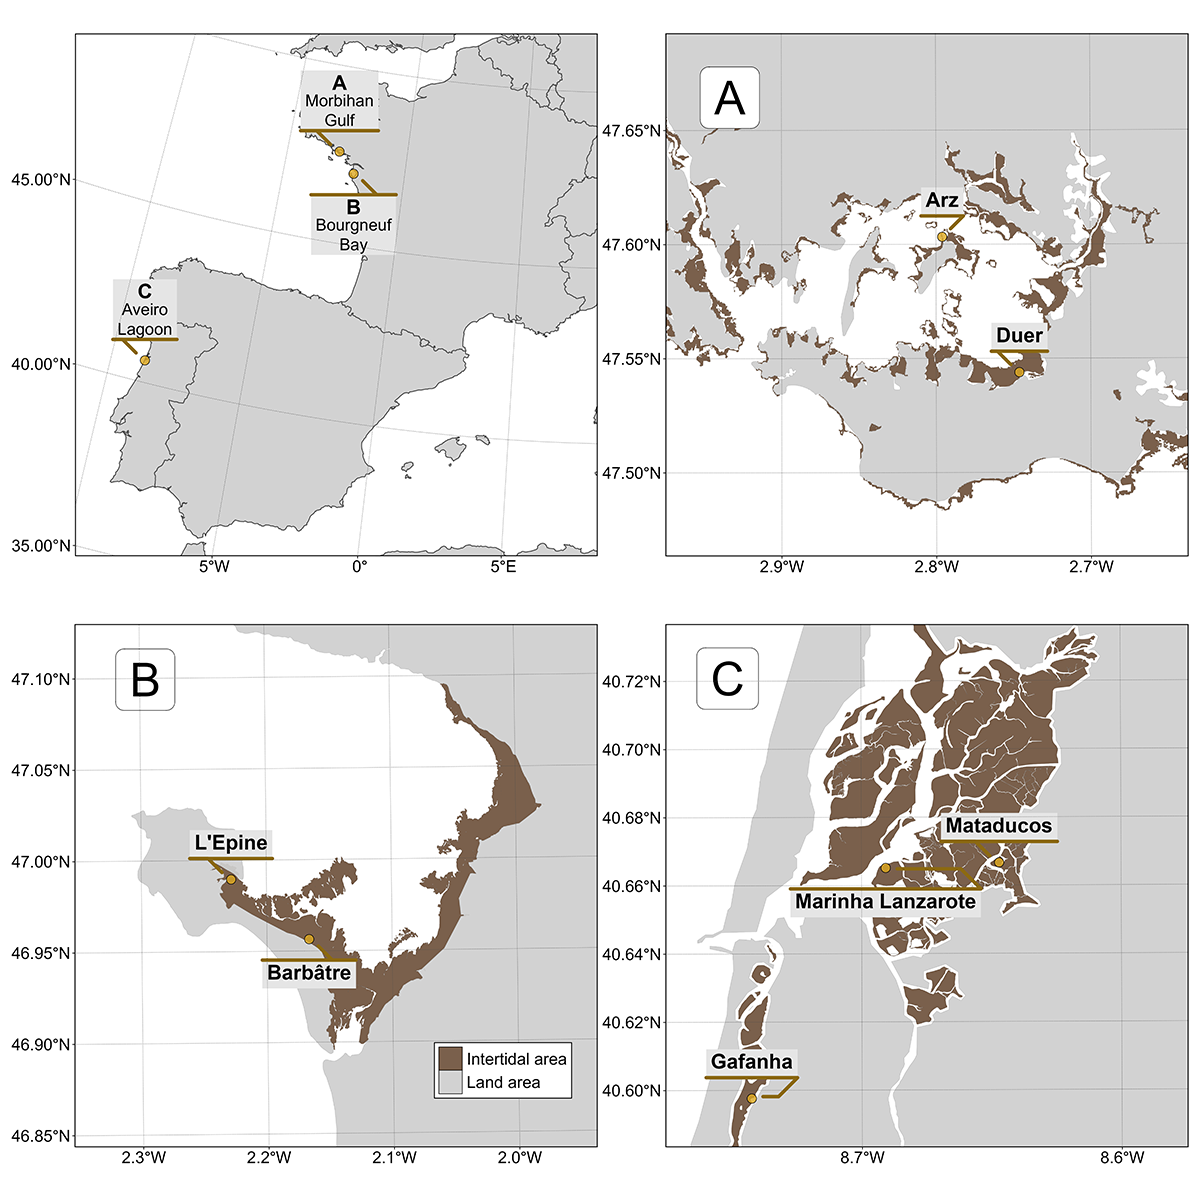
\includegraphics[width=1\textwidth,height=\textheight]{./Figures/Low_res/Fig1_Map_Drone_Sites.png}

}

\caption{\label{fig-map}Location of drone flights in France and
Portugal. A: Gulf of Morbihan (Two sites), B: Bourngeuf Bay (Two sites),
C: Ria de Aveiro Coastal Lagoon (Three sites). Green areas represents
the intertidal zone.}

\end{figure}%

\subsection{Field sampling}\label{field-sampling}

\subsubsection{Drone acquisition}\label{drone-acquisition}

At each location, a DJI Matrice 200 quadcopter drone equipped with a
Micasense RedEdge Dual MX multispectral camera was flown to take 1.2
million pixel reflectance photographs with ten spectral bands ranging
from the blue to the near infrared (NIR): 444, 475, 531, 560, 650, 668,
705, 717, 740 and 840 nm. To ensure consistent lighting conditions
across flight paths, the drone's trajectory was aligned to maintain a
solar azimuth angle of 90 degrees. An overlap of 70\% and 80\% (side and
front respectively) between each image was set for each flight. A
downwelling light sensor (DLS2) was used to acquire irradiance data
concomitantly with the camera measurements. Raw data were calibrated in
reflectance using a calibration panel reflective at \textasciitilde50\%
provided by the manufacturer. Across all sites, flights were made at two
different altitudes : 12 m or/and 120 m. (Table~\ref{tbl-flights}).

\begin{table}

\caption{\label{tbl-flights}List of drone flight, summarising the date,
the altitude, and the purpose of each flight. 12 m and 120 m flights
have a spatial resolution of 8 and 80 mm respectively.}

\centering{

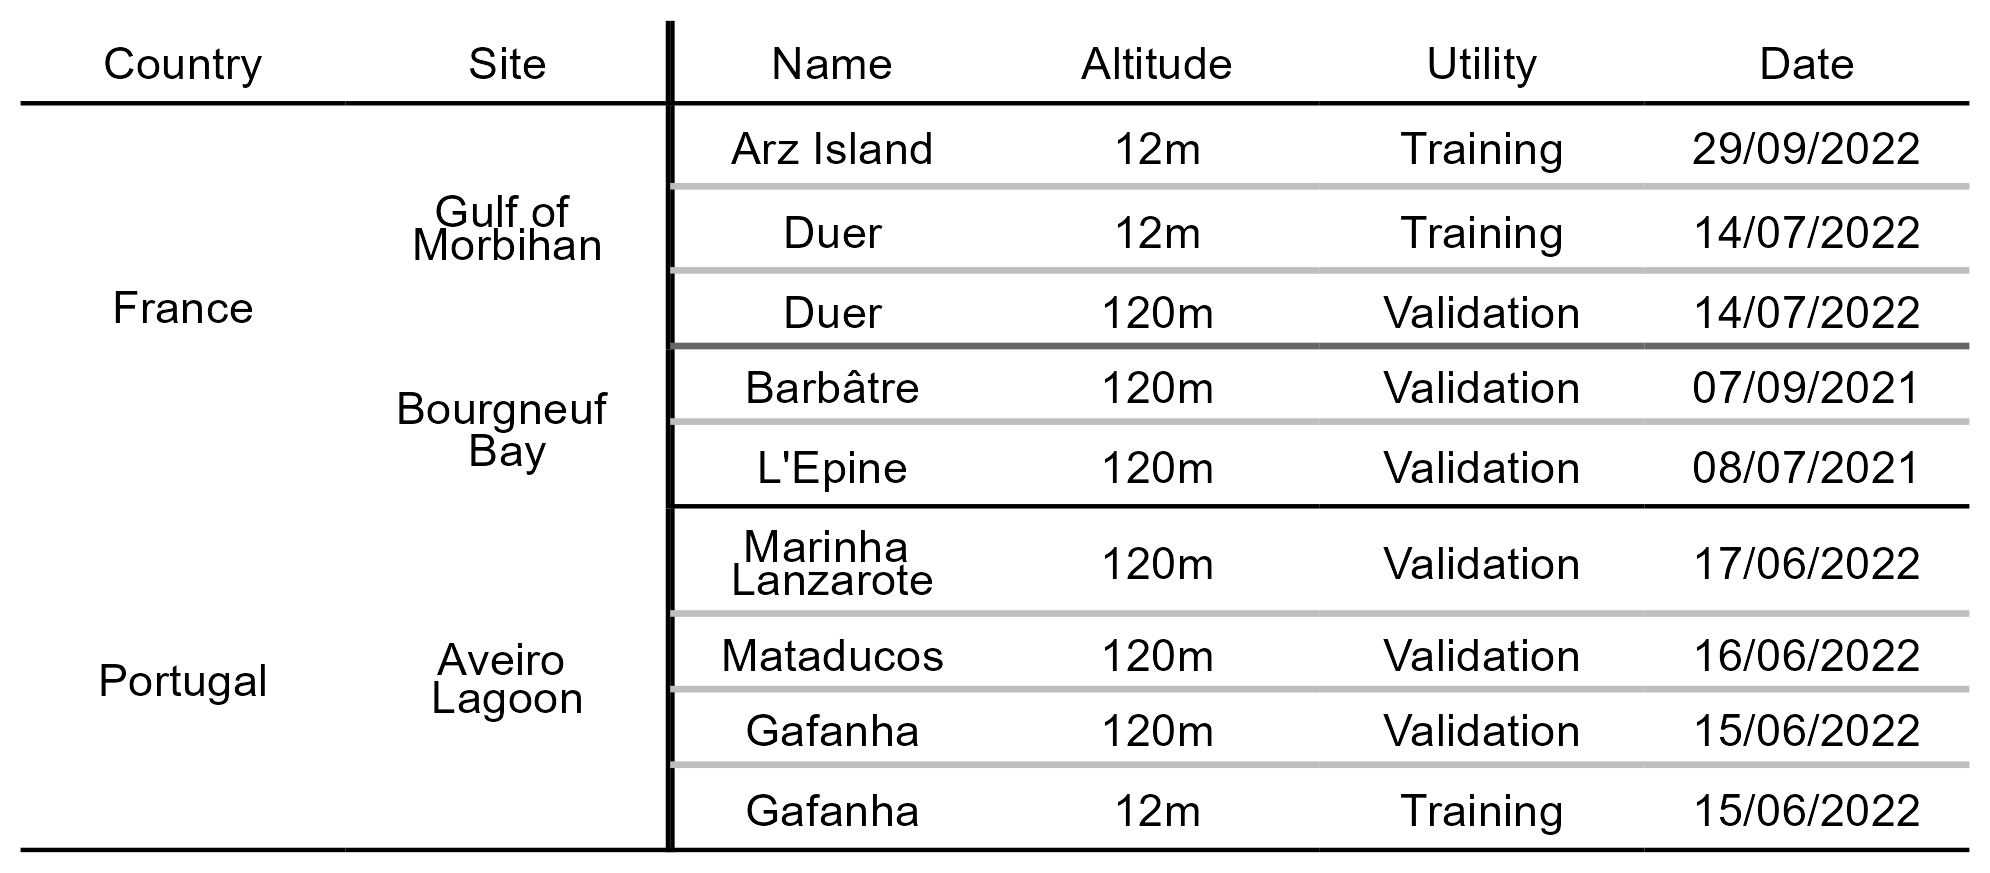
\includegraphics[width=6.63in,height=\textheight]{Figures/High_res/Table1/table_flights.png}

}

\end{table}%

\subsubsection{Ground Control Points}\label{ground-control-points}

Before each flight, targets used as ground control points were
distributed over the study site and georeferenced with a Trimble © Geo
XH 6000 differential GPS (dGPS). Ground control points were used to
correct georeferencing imprecision of orthomosaics with an horizontal
and vertical accuracy of 10cm. A dGPS was also used to georeference
quadrats of 0.25 m² ,which assessed the presence or absence of five key
taxonomic classes of intertidal vegetation : Bacillariophyceae
(unicellular benthic diatoms forming biofilms at the sediment surface
during low tide), Phaeophyceae (brown macroalgae), Magnoliopsida (dwarf
eelgrass), Chlorophyceae (green macroalgae) and Rhodophyceae (red
macroalgae) (Figure~\ref{fig-vegetation}). Pictures of each quadrat were
uploaded online to the Global Biodiversity Information Facility (GBIF)
platform \citep{BedeGbif}, a public open portal to store and share
biodiversity data. Each photograph was also processed to estimate the
percent cover of each type of vegetation using an image processing
software \citep[ImageJ,][]{schneider2012nih}. Hyperspectral reflectance
signatures of each vegetation class were recorded using an ASD FieldSpec
HandHeld 2 spectroradiometer, which acquires reflectance between 325 and
1075 nm, with 1 nm of spectral resolution. Hyperspectral signatures
served dual purposes: they validate the radiometric calibration of drone
data and contribute to error reduction in photo interpretations.

\phantomsection\label{cell-fig-vegetation}
\begin{figure}[H]

\centering{

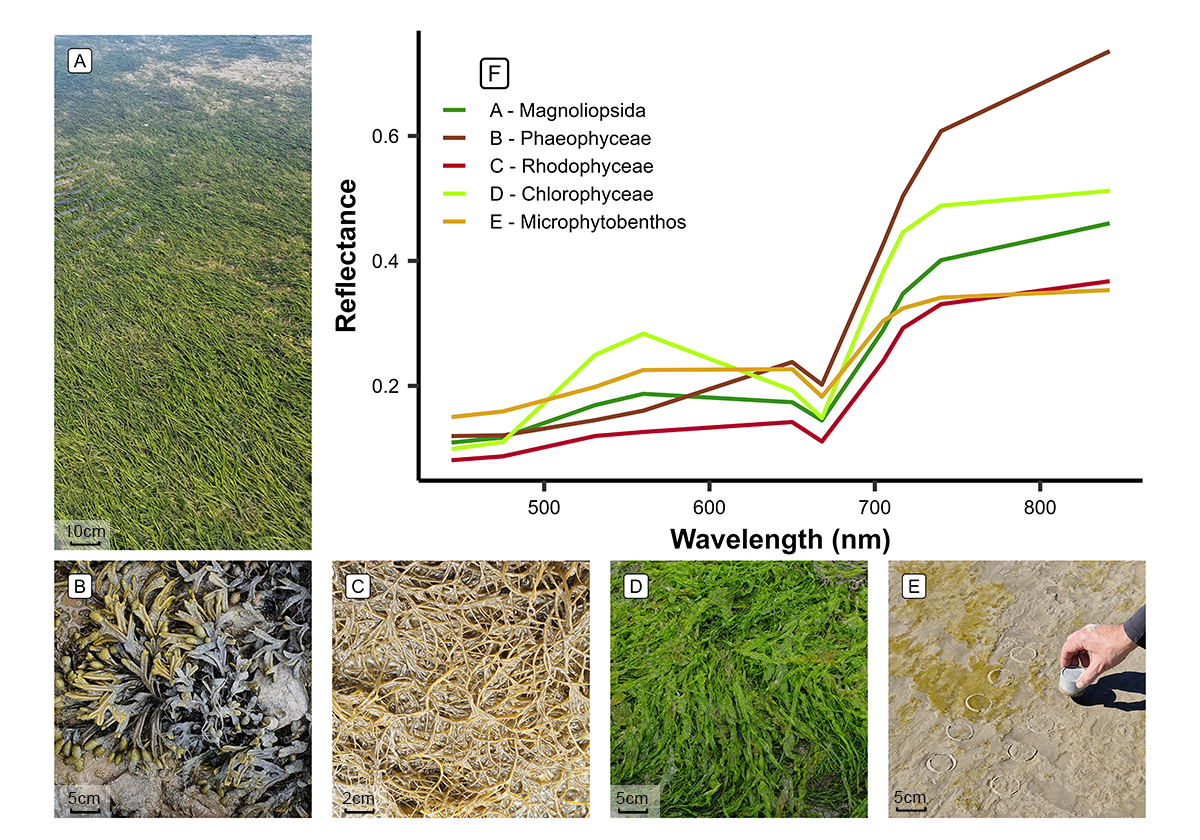
\includegraphics[width=1\textwidth,height=\textheight]{Figures/Low_res/Spectral_shapes_total.png}

}

\caption{\label{fig-vegetation}The five taxonomic classes of vegetation
used to train the Neural Network model and their raw spectral signatures
at the spectral resolution of the Micasense RedEdge Dual MX. A :
Magnoliopsida (Nanozostera noltei syn. Zostera noltei) ; B :
Phaeophyceae (Fucus sp.) ; C : Rhodophyceae (Gracilaria vermiculophylla)
; D : Chlorophyceae (Ulva sp.) ; E : Bacillariophyceae (Diatoms - MPB)}

\end{figure}%

\subsection{Drone Processing}\label{drone-processing}

A structure-from-motion photogrammetry software \citep[Agisoft
Metashape,][]{agisoft}was used to process images to obtain multispectral
orthomosaics of each flight. The process for orthomosaicking was
identical for every flight. First, tying key points were detected inside
of each image and between overlapping images in order to obtain a sparse
point cloud. This cloud was cleaned using reprojection accuracy metric
in order to remove noisy points. A dense point cloud was then produced
using a structure from motion algorithm. A surface interpolation of this
dense point cloud was made to obtain a digital surface model (DSM), used
to reconstruct the multispectral ortho-image \citep{nebel2020review}.
Low altitude drone flights produced ortho-images with a very high
spatial resolution (8 mm per pixel), making it efficient to visually
distinguish between the various types of vegetation. High altitude
flights on the other hand allowed to cover large areas and produced
images with a pixel size of 80 mm (Table~\ref{tbl-flights}).

\subsection{General Workflow}\label{general-workflow}

The spectral similarities of the reflectance signatures between
intertidal green macrophytes (Magnoliopsida and Chlorophyceae) make
their discrimination challenging using simple classification algorithms
(Figure~\ref{fig-vegetation} F). To overcome this challenge, a deep
learning classification method was trained, validated, and applied to
each drone flight (Figure~\ref{fig-workflow}).

\phantomsection\label{cell-fig-workflow}
\begin{figure}[H]

\centering{

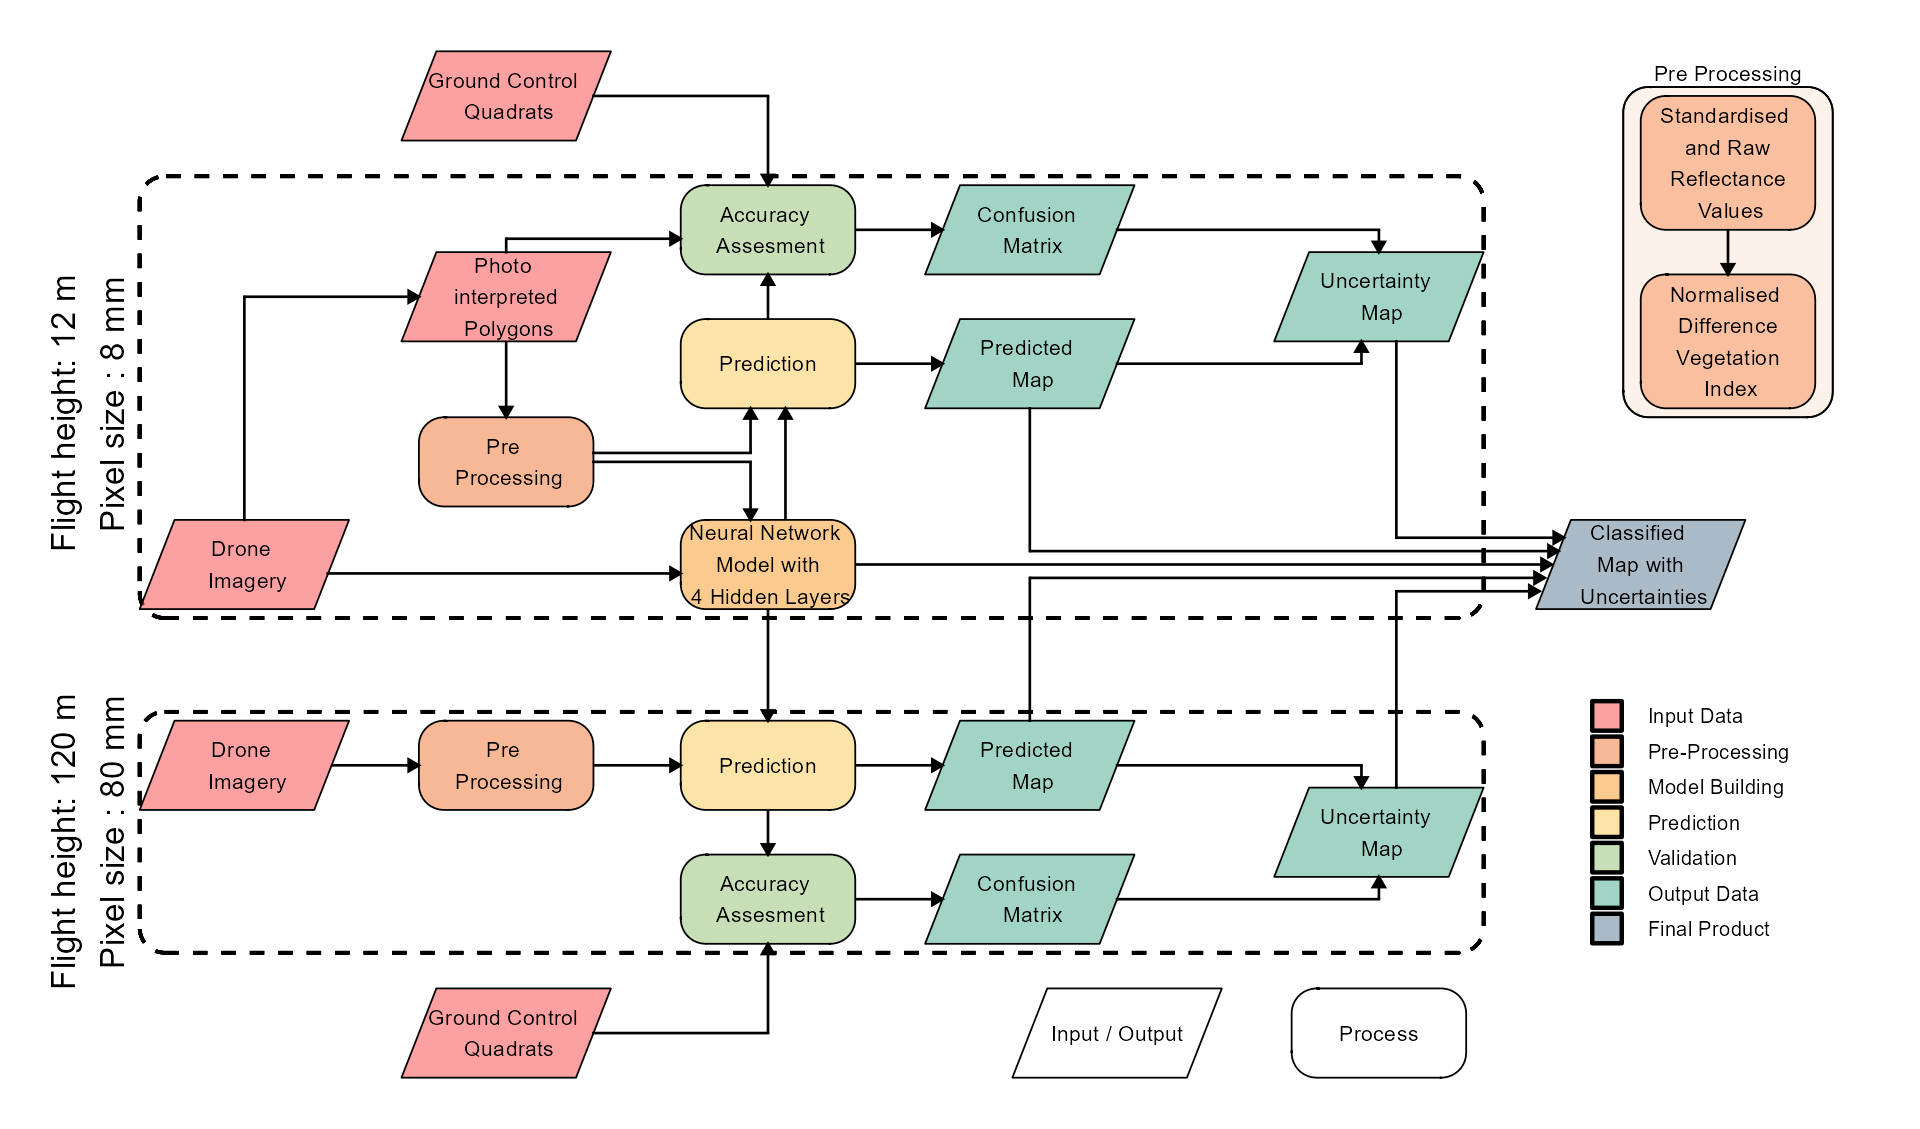
\includegraphics[width=1\textwidth,height=\textheight]{./Figures/Low_res/Figure3_workflow.png}

}

\caption{\label{fig-workflow}Schematic representation of the workflow.
Parallelograms represent input or output data, and rectangles represent
Python processing algorithms. The overall workflow of this study is
divided into two distinct parts based on the spatial resolution of the
drone flights: high-resolution flights (pixel size: 8 mm) were utilized
for training and prediction of the Neural Network model, whereas
lower-resolution flights (pixel size: 80 mm) were solely employed for
prediction purposes. Validation has been performed on both high and low
resolution flights.}

\end{figure}%

\subsubsection{Training dataset
building}\label{training-dataset-building}

\begin{table}

\caption{\label{tbl-validationPX}Vegetation Classes of the model and the
number of pixels used to train and validate each class}

\centering{

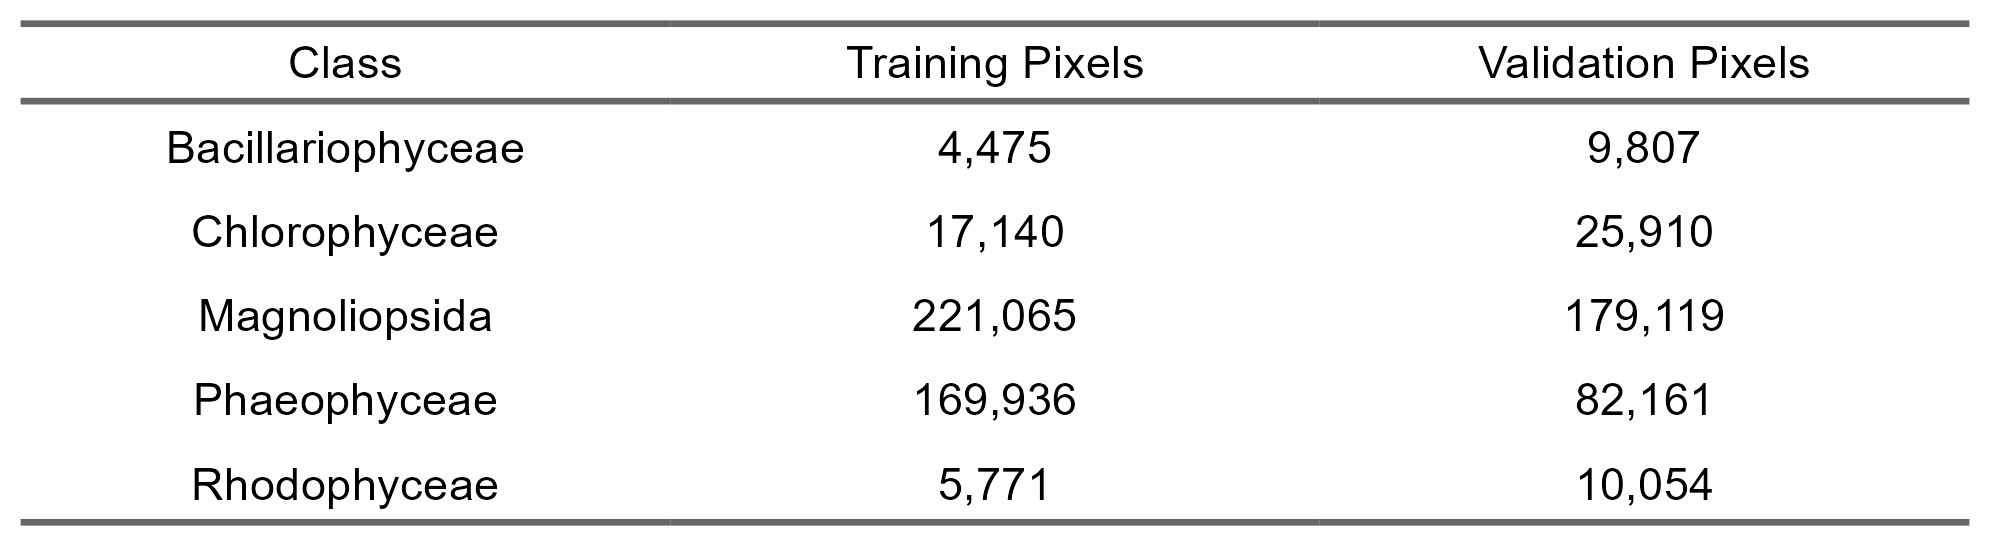
\includegraphics[width=6.63in,height=\textheight]{Figures/High_res/table_validation_px.png}

}

\end{table}%

A dataset containing photo-interpreted drone reflectance pixels was
built to train a Neural Network model. The training pixels were
categorized into seven different classes, representing the various
habitats encountered at the different study sites: Sediment, Water,
Chlorophyceae, Magnoliopsida, Bacillariophyceae, Phaeophyceae and
Rhodophyceae. Only low-altitude flights (Table~\ref{tbl-flights}) were
used for training because their 8 mm spatial resolution allowied to
avoid spectral sub-pixel mixing and to accurately identify vegetation
classes. More than 418,000 pixels at 8 mm resolution from the 3 training
flights were used to train the model (Table~\ref{tbl-validationPX}).
Twenty one variables were used by the model as predictors: the ten raw
spectral bands of the Micasense RedEdge Dual MX multispectral camera
(ranging from 444 nm to 840 nm), the same ten spectral bands
standardized using a min/max transformation (Equation~\ref{eq-std} ;
\citep{Cao2017}) and the Normalized difference vegetation index (NDVI,
Equation~\ref{eq-ndvi}). Standardisation of spectral bands is commonly
used to eliminate the scaling differences between spectra and to limit
the effect of biomass on the spectra shape \citetext{\citealp[
]{Douay2022}; \citealp{Davies2023}}.

\begin{equation}\phantomsection\label{eq-std}{
R_{i}^{*}(\lambda) = \frac{R_{i}(\lambda) - min(R_{i})}{max(R_{i})- min(R_{i})}
}\end{equation}

where \(R_{i}(\lambda)\) is the reflectance at the wavelength
\((\lambda)\) of each individual spectra \((i)\), \(min(R_{i})\), and
\(max(R_{i})\) are the minimum and maximum value of the spectra \((i)\)

\begin{equation}\phantomsection\label{eq-ndvi}{
NDVI = \frac{R(840nm)-R(668nm)}{R(840nm)+R(668nm)}
}\end{equation}

where \(R(840nm)\) is the reflectance at 840 nm and \(R(668nm)\) is the
reflectance at 668 nm.

\subsubsection{Model building}\label{model-building}

A neural network classification model was built using the fastai
workflow \citep{howard2018fastai}. This model is composed by 2 hidden
layers and have a total of 26 054 trainable parameters. Parameters have
been find tune using 12 epoch to minimize the error rate.

\subsubsection{Validation}\label{validation}

The workflow of this study revolves around two distinct flight heights
(12 m and 120 m, Figure~\ref{fig-workflow}) where ensuring consistency
between reflectances at both heights is crucial. This comparison was
conducted at sites where low and high altitude flights overlapped. The
low altitude flights were resampled to the same spatial resolution and
grid as the high flights using a median resampling method. Reflectance
values were then extracted, and a scatterplot was generated.
Subsequently, the slope of the linear model and the coefficient of
determination (R²) were computed.

The model was applied to all flights at both 12 and 120 m of altitude.
In situ information on georeferenced class type and percent cover
collected during each flight was used to assess the model accuracy.
These images were used to construct a validation dataset indicating the
presence or absence of each class. Additionally to the quadrat-based
validation dataset, polygons of each class were photo interpreted in
order to increase the number of pixels of the validation dataset.A total
of 536,000 pixels were used to validate the Neural Network classifier.
The sites with the lowest and highest number of validation data were
Gafanha Low (17316 pixels) and Marinha Lanzarote (159713 pixels),
respectively.A confusion matrix, along with precision metrics such as
global accuracy, sensitivity, specificity, and Kappa coefficient, was
generated for each sites. All validation matrices were then aggregated
to create an overall matrix .

\subsection{Variable Importance}\label{variable-importance}

Variable Importance Plots (VIP) serve as a method to identify which
predictors are important for predicting a specific class. Out of the
twenty one predictors utilized in this study, Variable Importance was
computed only for the raw and standardized values of the 10 spectral
bands captured by the MicaSense camera. This is achieved by repeatedly
predicting the same dataset while randomly shuffling one predictor at a
time. The benchmark score obtained after each iteration is then compared
to the benchmark score obtained without shuffling any variables. The
greater the difference between these two benchmark values, the more
important the variable is for the model \citep{WEI2015399}.

\subsection{Impact of the spatial resolution in the
prediction}\label{impact-of-the-spatial-resolution-in-the-prediction}

To assess the impact of spatial resolution on the model's output, the
reflectance of each flight's orthomosaic was spatially resampled using
the average method from the Terra package in R. DISCOV was then applied
to these resampled rasters. The results were compared to the original
model predictions, which were resampled using the mode method from the
Terra package in R. For each resolution and each class of the model, an
agreement percentage was obtained, where a score of 100 indicates that
all pixels in the two products are identical, and a score of 0 indicates
that all pixels are different.

We used a Generalized Linear Model (GLM) with a Gaussian family and an
identity link function to investigate the relationship between pixel
resolution, vegetation class, and their interaction on the response
variable, the agreement. The formula for the model was:

\begin{equation}\phantomsection\label{eq-gam}{
Agreement \sim  Resolution \times VegetationClass
}\end{equation}

\subsection{Impact of the vegetation cover on the
prediction}\label{impact-of-the-vegetation-cover-on-the-prediction}

The key aspect of the workflow adopted in the present study is the
mapping of specific areas at two different altitudes (12m and 120m),
resulting in two distinct resolutions for the same area (8mm and 80mm).
The predictions made on the high-resolution flight can be used to
estimate the cover (percentage, \%) of each vegetation class for every
pixel of the lower resolution flight. Consequently, for each pixel of
the high-altitude flights, the cover (\%) of each vegetation class were
obtained, and a kernel density plot was generated. This plot provides a
visual representation of the behavior of the model in different
vegetation percent cover scenarios.

\section{Results}\label{results}

\subsection{Classification}\label{classification}

Each drone flight was used to produce a prediction map, as well as a
probability map that indicates the model derived likelihood of the
selected class for every pixel. The low-altitude flight conducted in
Gafanha, Portugal, represents the site with the highest complexity
(Figure~\ref{fig-GafLow}). Among the five vegetation classes on which
the model was trained, four were present on this site, with
Chlorophyceae and Rhodophyceae mixed with the seagrass meadow. There was
also Bacillariophyceae forming biofilms on parts of bare sediment
surface. Although the seagrass bed was solely composed of
\emph{Nanozostera noltei}, various colors of this specie could be
observed from dark green (corresponding to healthy leaves) to
whitish/brown (when leaves were discolored having lost their
pigmentation). Regardless of color, Magnoliopsida pixels were accurately
predicted by the model.

\phantomsection\label{cell-fig-GafLow}
\begin{figure}[H]

\centering{

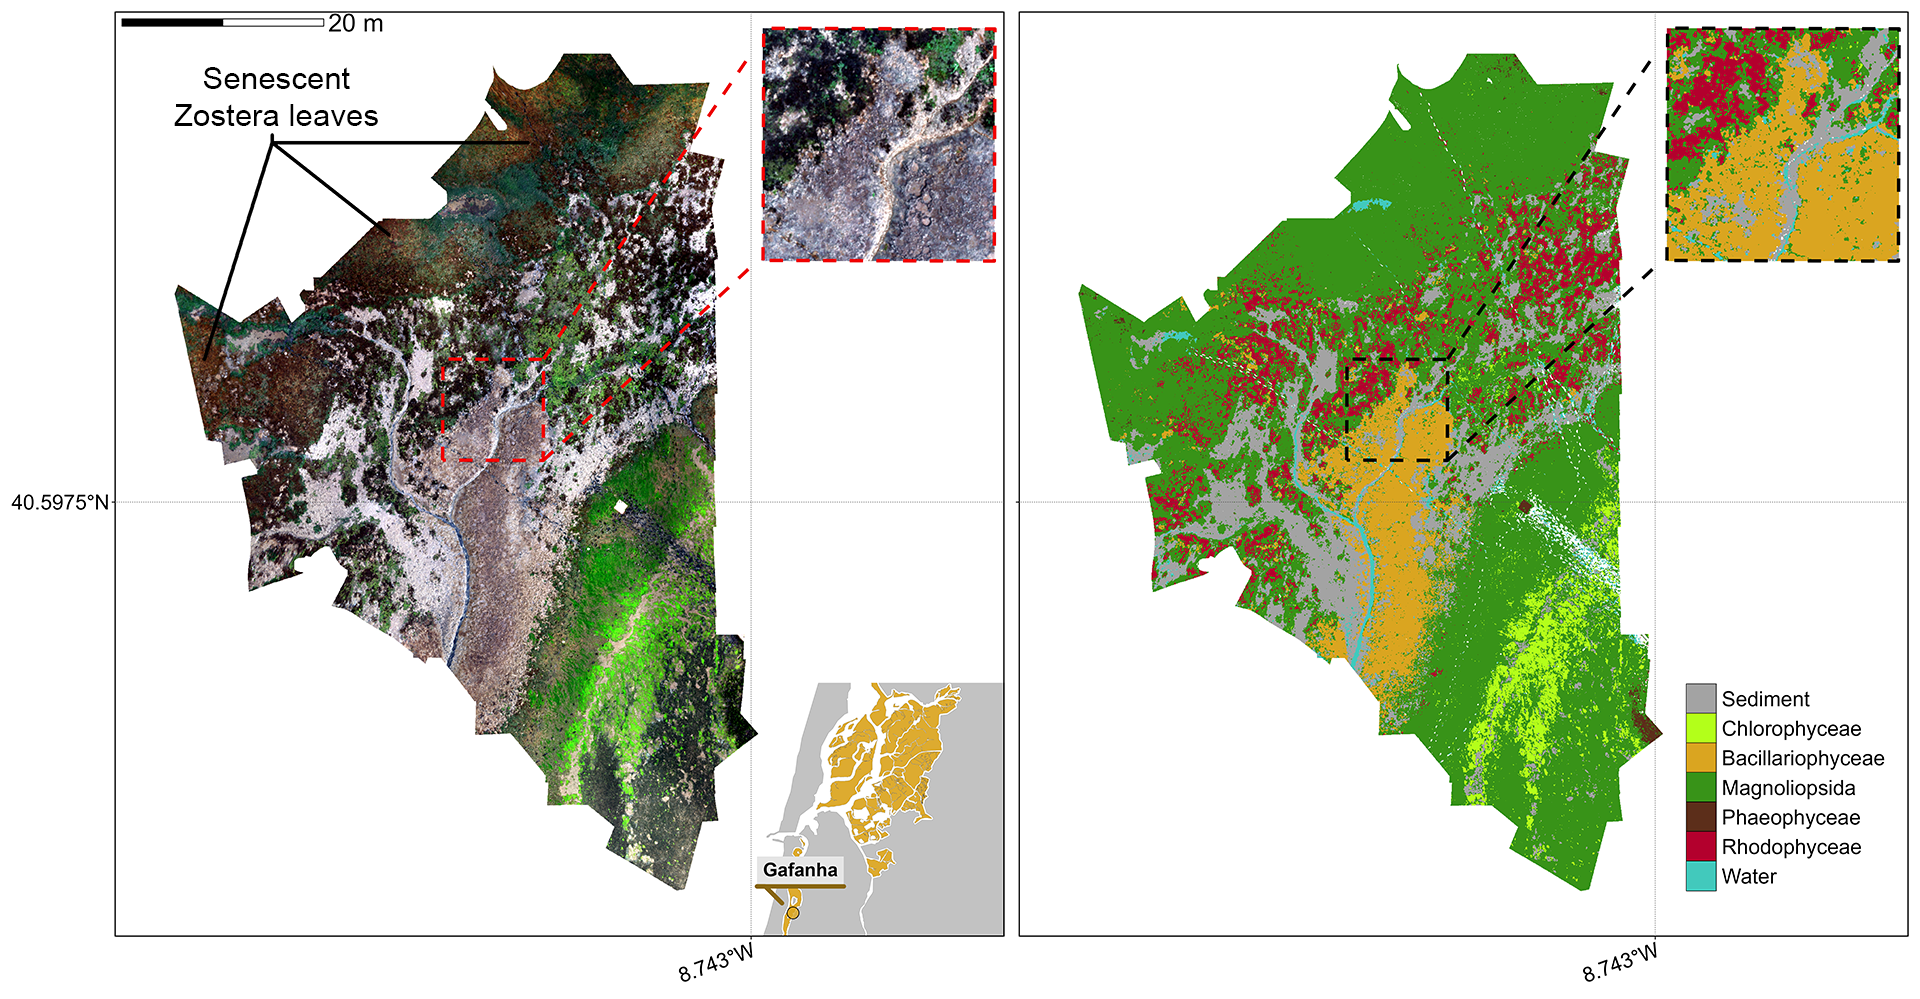
\includegraphics[width=1\textwidth,height=\textheight]{./Figures/Low_res/Maps Pred/FigX-Gaf_Low_Pred.png}

}

\caption{\label{fig-GafLow}RGB orthomosaic (Left) and Prediction (Right)
of the low altitude flight of Gafanha, Portugal. The total extent of
this flight was 3000 m² with a resolution of 8 mm per pixel. Background
colors indicate intertidal area (Light Green) and land area (Light
Grey). The zoom covers an area equivalent to a 10-meter Sentinel-2 pixel
size.}

\end{figure}%

The high-altitude flight over Gafanha covered a total area of
\textasciitilde1 km² (Figure~\ref{fig-GafHigh}). A channel contouring a
small island was masked in the prediction map. Most of the intertidal
area was classified as Magnoliopsida by the model, including seagrass
patches with discolored leaves. Only a few pixels were classified as
Chlorophyceae at this spatial scale. Furthermore, the area that was
classified as Bacillariophyceae in the low-altitude flight remained
mostly classified as such in the high-altitude flight, though some
pixels were classified as Magnoliopsida. Patches of Rhodophyceae were
correctly classified. In the northern part of the site and near the land
eadges, patches of the schorre angiosperm \emph{Sporobolus maritimus}
(syn. \emph{Spartina maritima)} were misclassified, either as
Magnoliopsida or as Phaeophyceae.

\phantomsection\label{cell-fig-GafHigh}
\begin{figure}[H]

\centering{

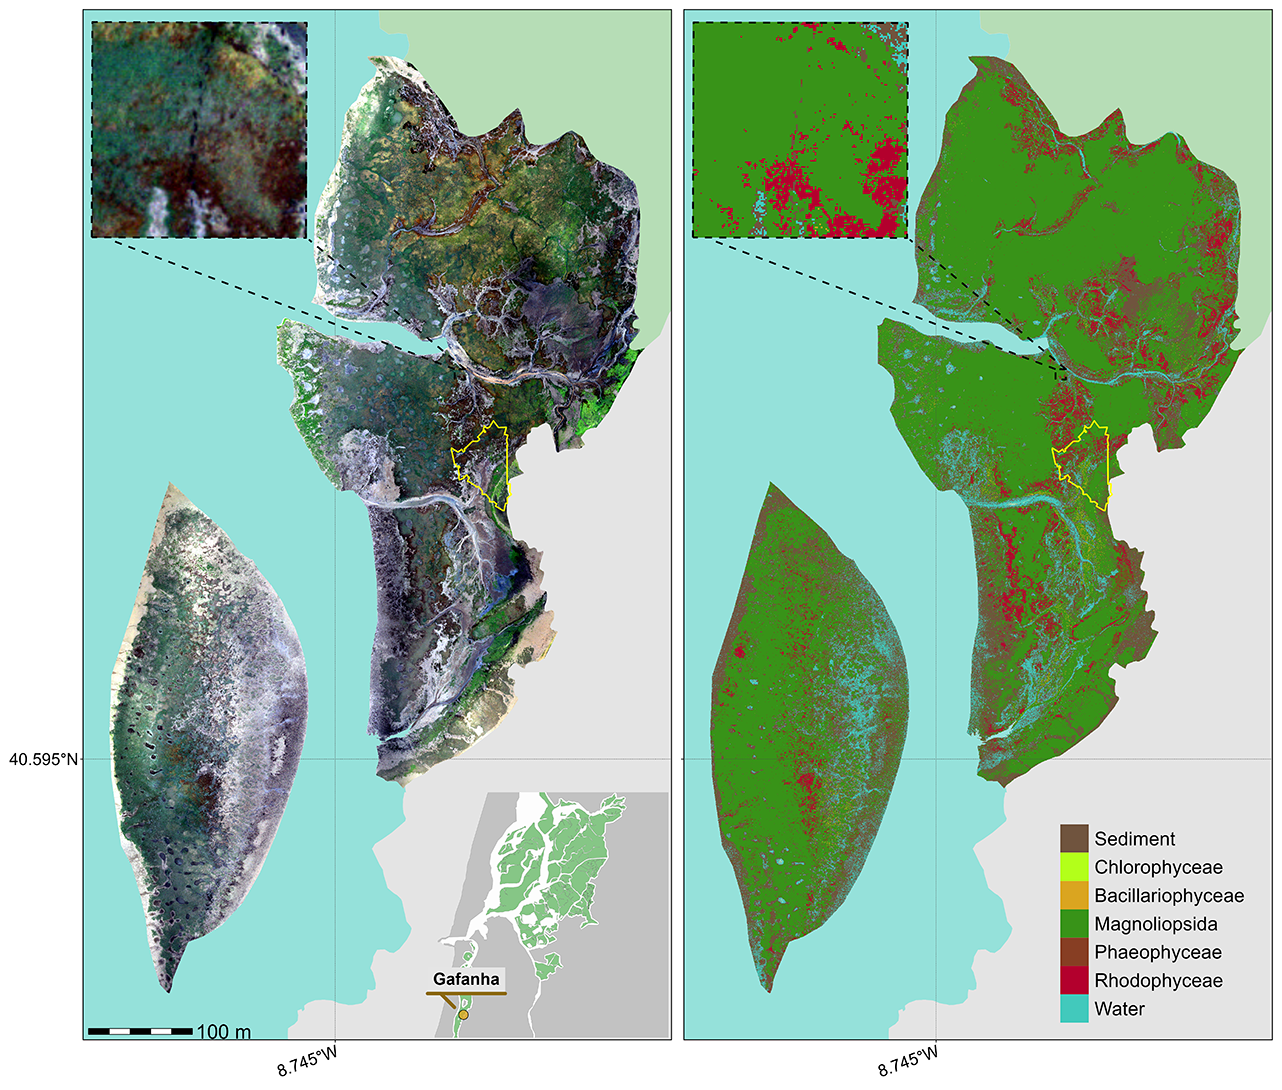
\includegraphics[width=1\textwidth,height=\textheight]{./Figures/Low_res/Maps Pred/FigX-Gaf_High_Pred.png}

}

\caption{\label{fig-GafHigh}RGB orthomosaic (Left) and Prediction
(Right) of the high altitude flight of Gafanha, Portugal. The total
extent of this flight was about 1 km² with a resolution of 80 mm per
pixel. Background colors indicate intertidal area (Light Green), land
area (Light Grey) and water (Light Blue). The yellow outline shows the
extent of the low altitude flight of Gafanha presented in
Figure~\ref{fig-GafLow}. The zoom covers an area equivalent to a
10-meter Sentinel-2 pixel size.}

\end{figure}%

Amoung the high altitude flights, the one acquired over the inner part
of Ria de Aveiro coastal lagoon covered the largest area with
approximately 1.5 km² (Figure~\ref{fig-Boat}). This site was dominated
by seagrass and red macroalgae. The classification provided consistent
results, with a patchy seagrass meadow mixed with red macroalgae on the
eastern part of the site. As shown in the zoom (Figure~\ref{fig-Boat}),
the edges of the meadow visually appears to be colonised by green
macroalgae (\emph{Ulva sp.}), which the model agreed with.

\phantomsection\label{cell-fig-Boat}
\begin{figure}[H]

\centering{

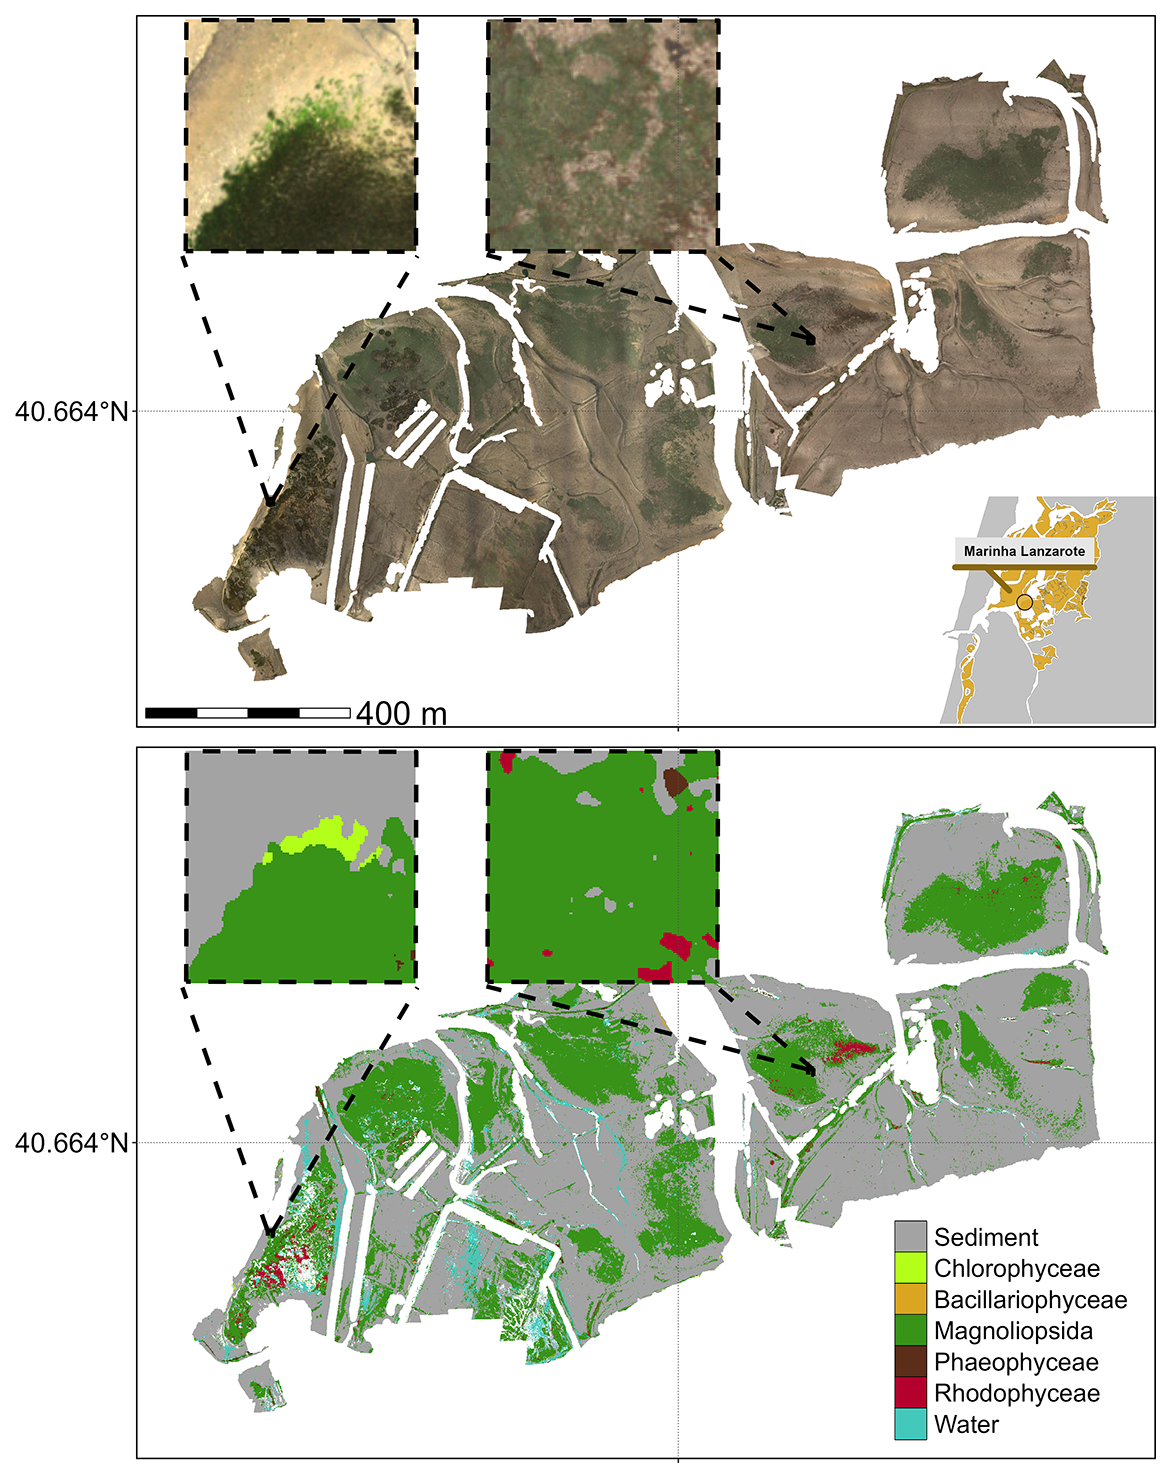
\includegraphics[width=1\textwidth,height=\textheight]{./Figures/Low_res/Maps Pred/FigX-Boat_Pred.png}

}

\caption{\label{fig-Boat}RGB orthomosaic (Top) and Prediction (Bottom)
of the flight made in the inner part of Ria de Aveiro Lagoon, Portugal.
The total extent of this flight was about 1.5 km² with a resolution of
80 mm per pixel. Background colors indicate intertidal area (Light
Green), land area (Light Grey) and water (Light Blue). Each cover an
area equivalent to a 10 m Sentinel-2 pixel size.}

\end{figure}%

The flight over L'Epine in Noirmoutier Island, France
(Figure~\ref{fig-Dike}) was conducted near a dike, which crossed the
northern part of the site from west to east. Alongside this dike, Fucale
brown algae (\emph{Fucus spp.}, \emph{Ascophyllum nodosum}) were
attached to sparse rocks and stranded green algae (\emph{Ulva spp.})
could be observed. Despite the high mixture between Chlorophyceae and
Magnoliopsida these two classes were correctly discriminated by the
classifier.

\phantomsection\label{cell-fig-Dike}
\begin{figure}[H]

\centering{

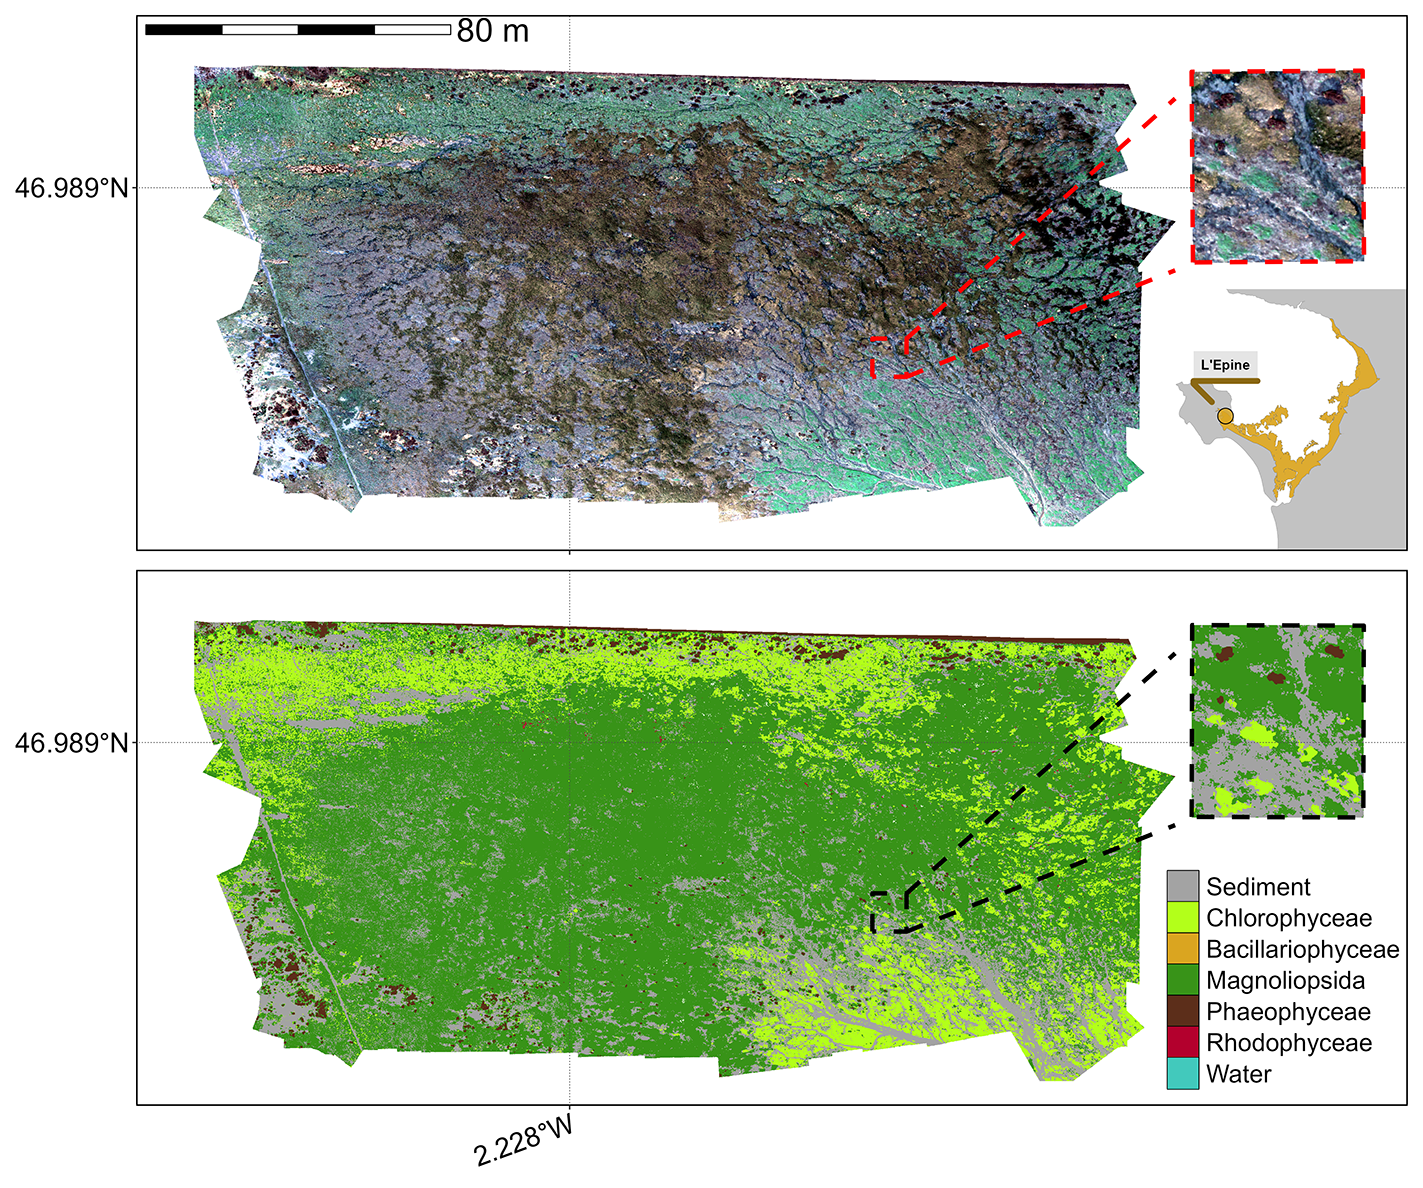
\includegraphics[width=1\textwidth,height=\textheight]{./Figures/Low_res/Maps Pred/FigX-Dike_Pred.png}

}

\caption{\label{fig-Dike}RGB orthomosaic (Top) and Prediction (Bottom)
of L'Epine, France. The total extent of this flight was about 28 000 m²
with a resolution of 80 mm per pixel. Background colors indicate
intertidal area (Light Green) and land area (Light Grey). The zoom
covers an area equivalent to a 10-meter Sentinel-2 pixel size.}

\end{figure}%

\subsection{Validation}\label{validation-1}

\subsubsection{Reflectance comparison between the two different
altitudes}\label{reflectance-comparison-between-the-two-different-altitudes}

In this study, a key innovation lies in the utilization of drone flights
at two different altitudes (12 m and 120 m) for constructing the neural
network model. Overall there was a good agreement between the two
altitudes (Figure~\ref{fig-CompareRef}).

\phantomsection\label{cell-fig-CompareRef}
\begin{figure}[H]

\centering{

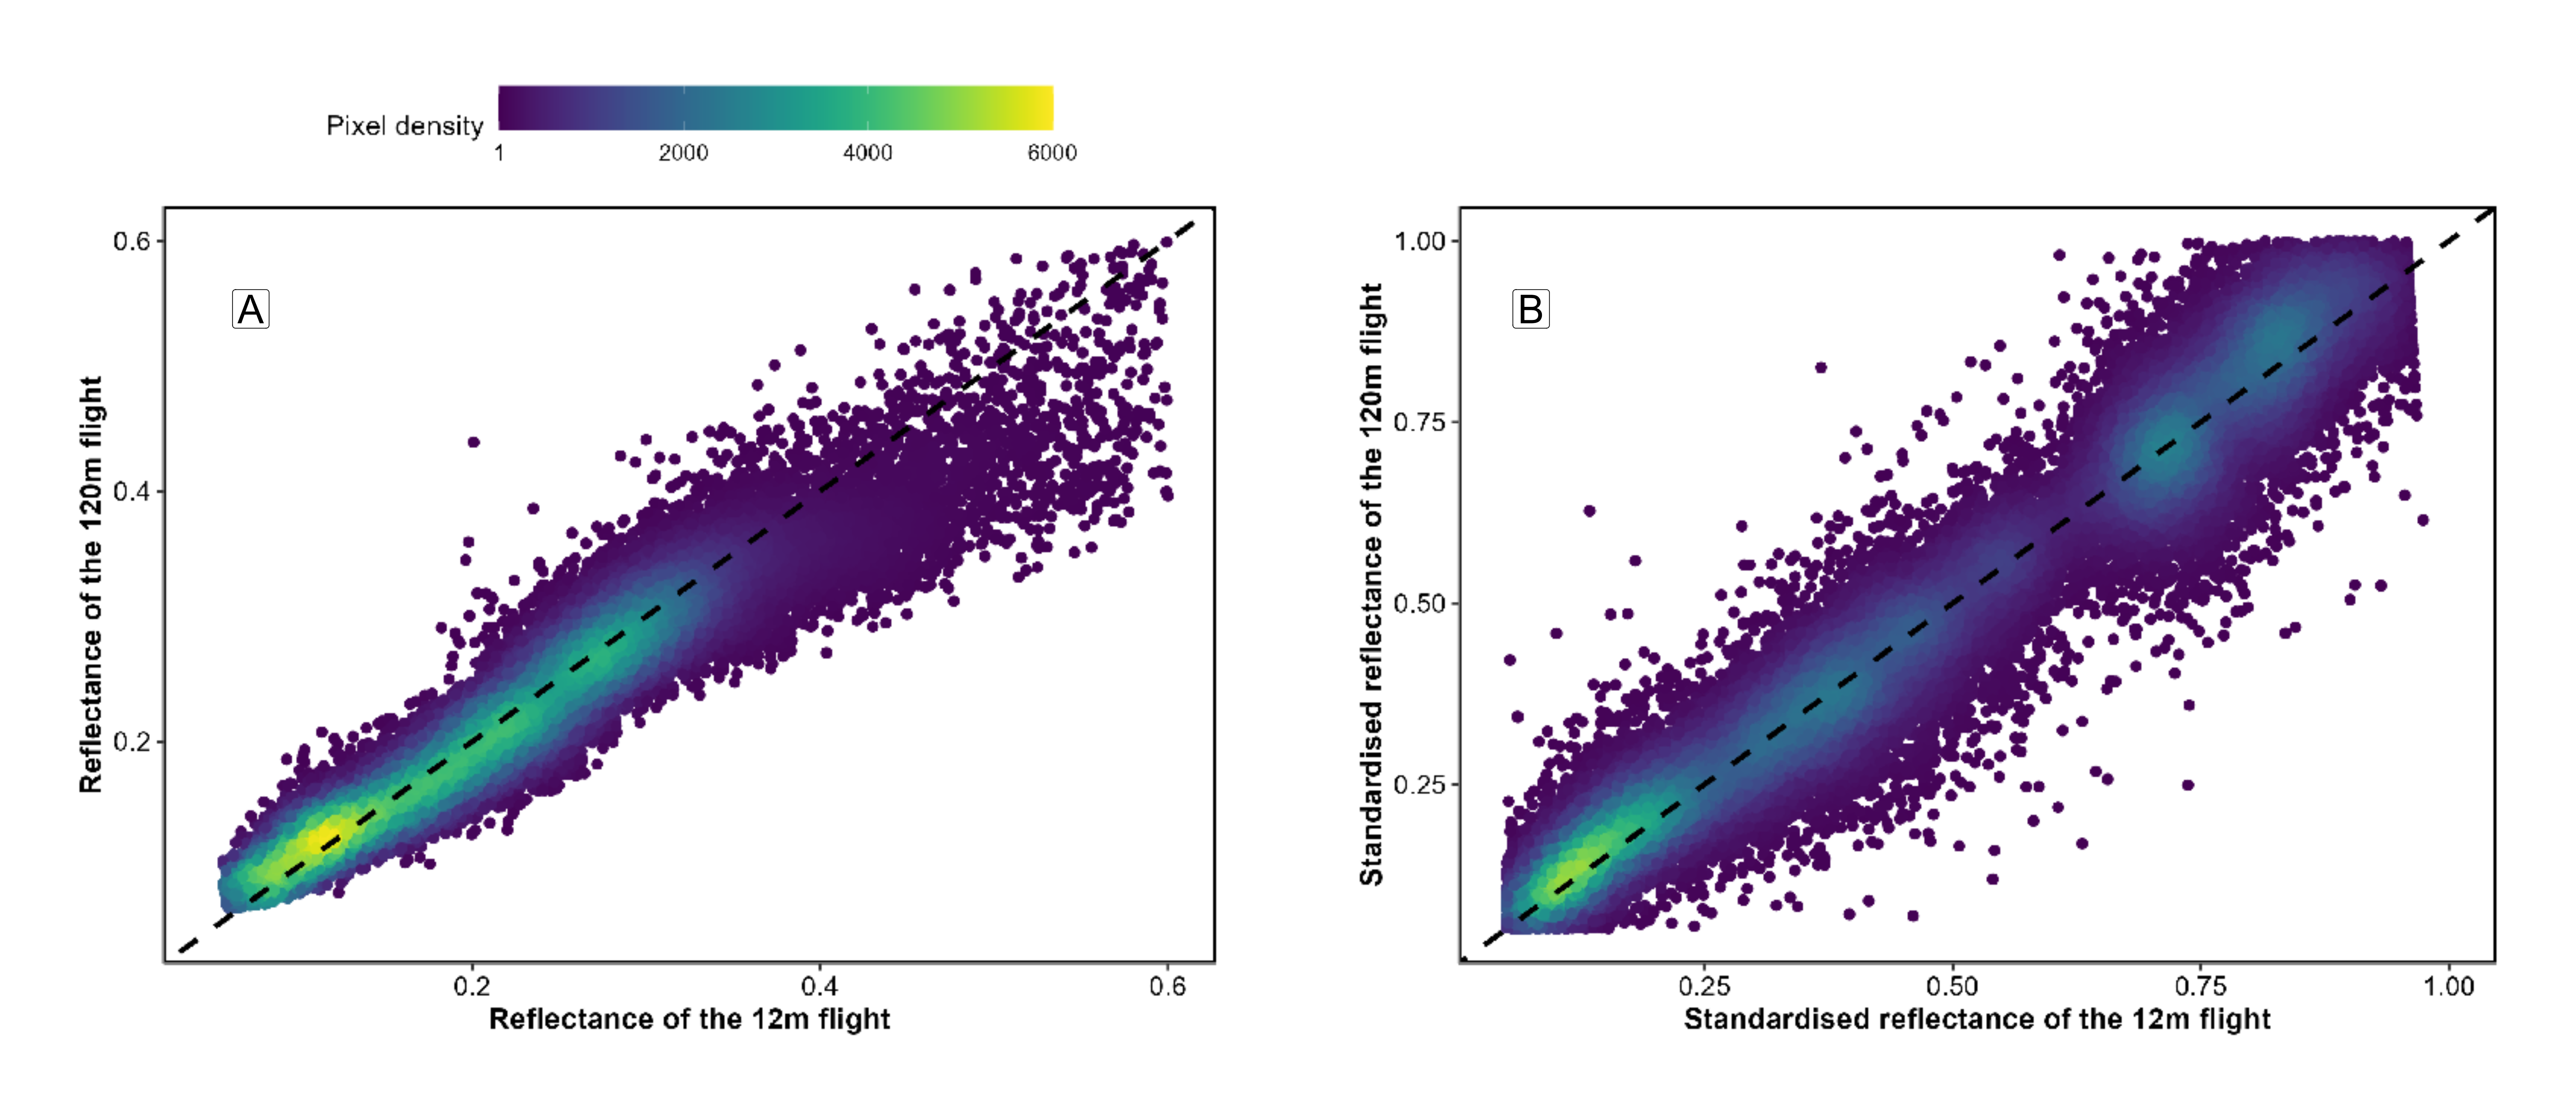
\includegraphics[width=1\textwidth,height=\textheight]{./Figures/High_res/Compare_reflectance_both.png}

}

\caption{\label{fig-CompareRef}Comparison of reflectance retrieved from
both low-altitude and high-altitude flights over a common area. The
black dashed line represents a 1 to 1 relationship. Left (A) plots raw
data and right (B) plots standardized data (Equation~\ref{eq-std}).}

\end{figure}%

There was a slight underestimation for raw reflectance values in the
high-altitude flight, particularly for higher reflectance values
(Figure~\ref{fig-CompareRef} A). Since both flights were conducted over
vegetation areas, the highest reflectance values correspond to the
infrared part of the spectrum. This difference is not present when
reflectance values have been standardized (Equation~\ref{eq-std} ;
Figure~\ref{fig-CompareRef} B).

\subsubsection{Neural network classification
validation}\label{neural-network-classification-validation}

Model global accuracy was 94.26\% with a Kappa coefficient of 0.92
(Figure~\ref{fig-Validation}).

\phantomsection\label{cell-fig-Validation}
\begin{figure}[H]

\centering{

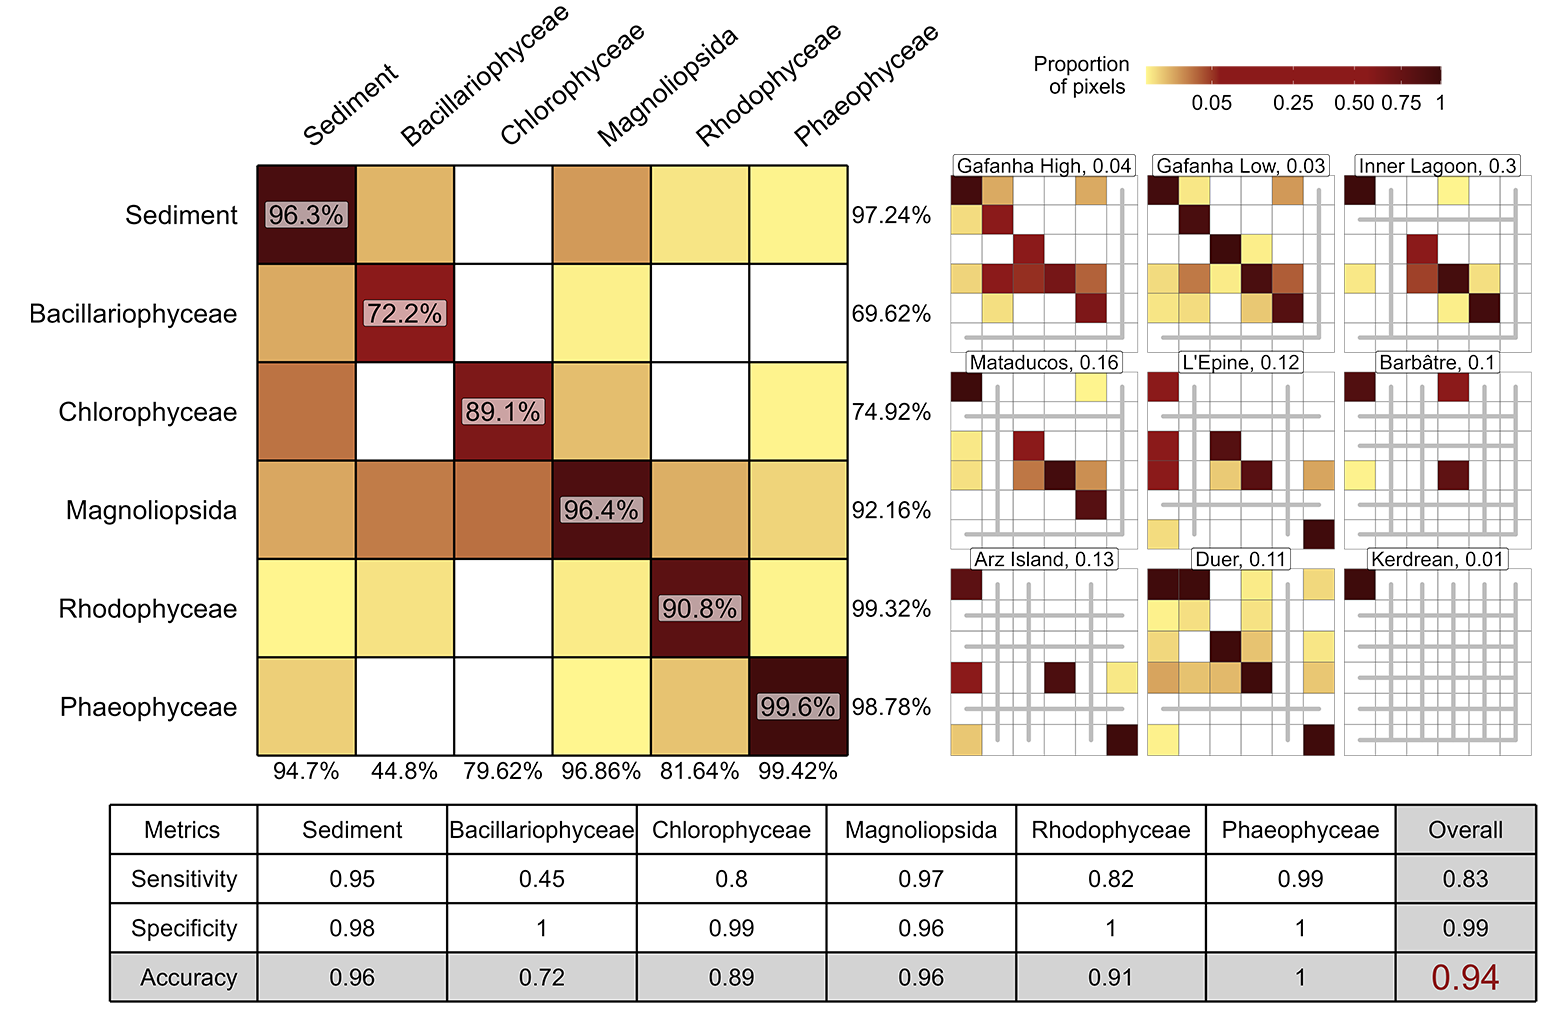
\includegraphics[width=1\textwidth,height=\textheight]{./Figures/Low_res/Validation/ConfusionMatrixGlobal.png}

}

\caption{\label{fig-Validation}A global confusion matrix on the left is
derived from validation data across each flight, while a mosaic of
confusion matrices from individual flights is presented on the right.
The labels inside the matrices indicate the balanced accuracy for each
class. The labels at the bottom of the global matrix indicate the User's
accuracy for each class, and those on the right indicate the Producer's
Accuracy. The values adjacent to the names of each site represent the
proportion of total pixels from that site contributing to the overall
matrix. Grey lines within the mosaic indicate the absence of validation
data for the class at that site. The table at the bottom summarizes the
Sensitivity, Specificity, and Accuracy for each class and for the
overall model.}

\end{figure}%

The lowest performing site was Gafanha High (global accuracy of 75.45\%)
whereas Mataducos was the site with the most accurate prediction (global
accuracy of 98.05\%). Overall, the classes Phaeophyceae, Magnoliopsida,
Sediment and Rhodophyceae were correctly classified with a balanced
accuracy of 1, 0.96, 0.96 and 0.91 respectively. Bacillariophyceae was
the least accurate class (accuracy of 0.72 ) mainly due to confusion
with Magnoliopsida and Sediment.

\subsection{Variable importance}\label{variable-importance-1}

The computation of the variable importance made it possible to identify
which bands were the most useful for class prediction
(Figure~\ref{fig-VIP}).

\phantomsection\label{cell-fig-VIP}
\begin{figure}[H]

\centering{

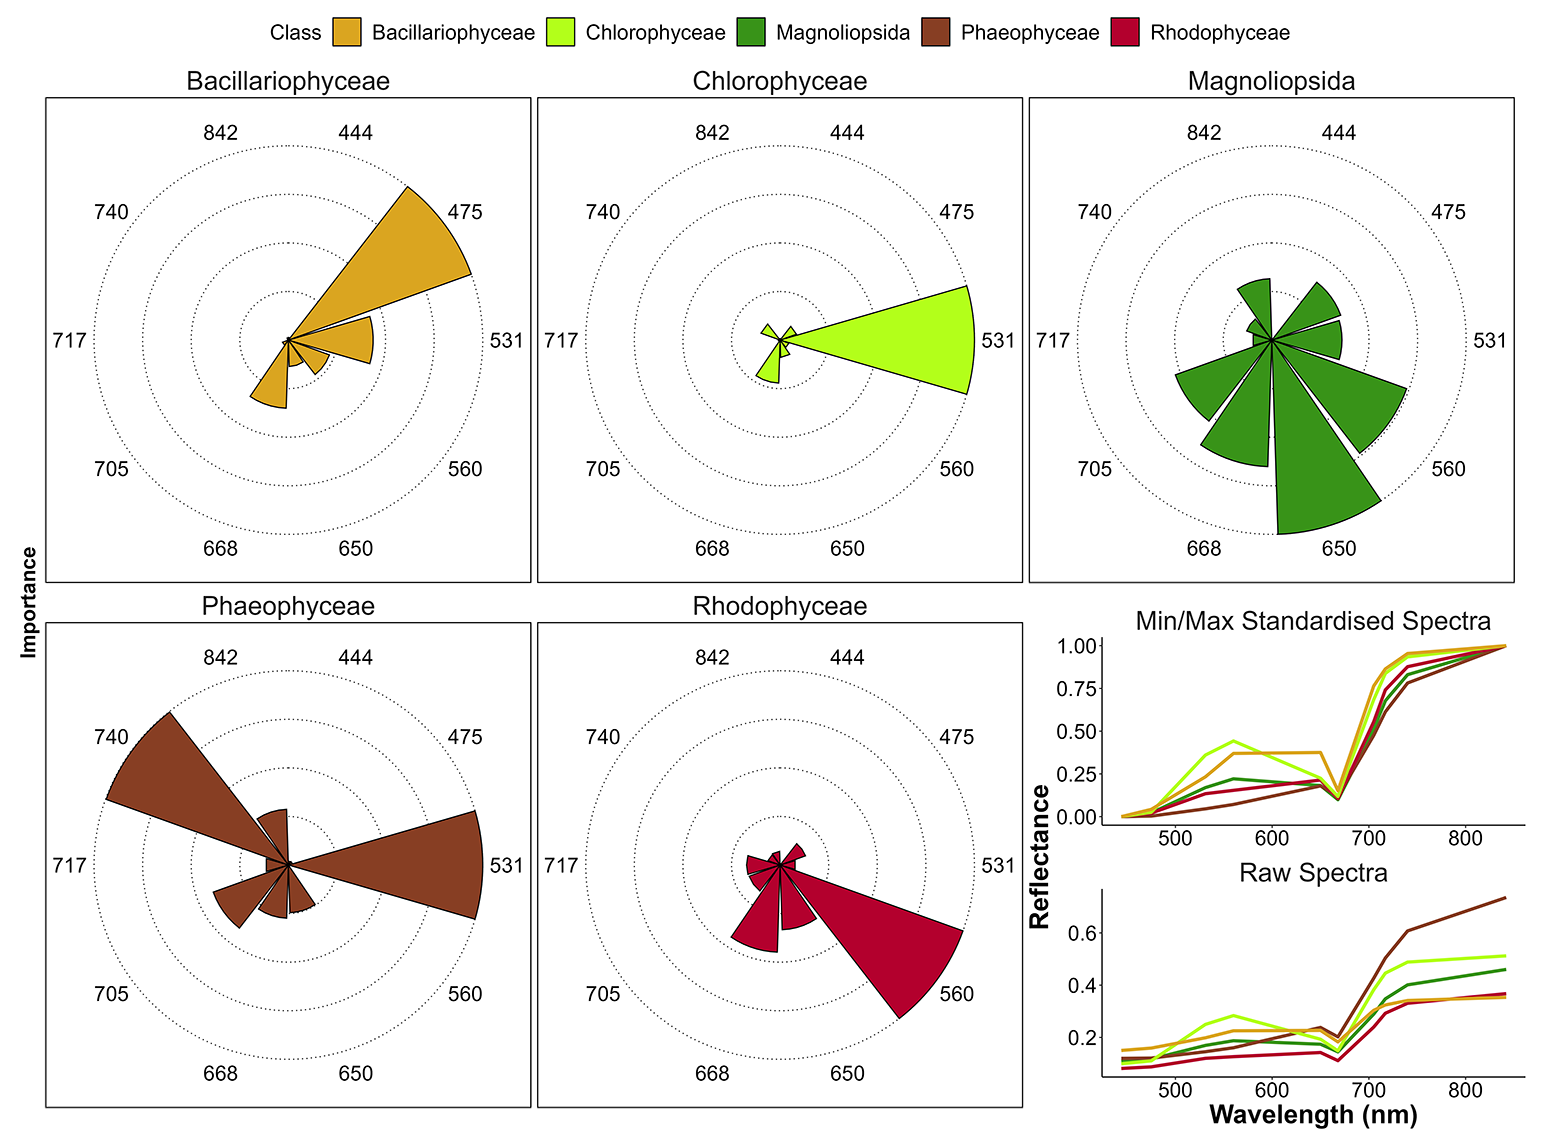
\includegraphics[width=1\textwidth,height=\textheight]{Figures/Low_res/VIP/Fig_VIP.png}

}

\caption{\label{fig-VIP}Variable Importance of the Neural Network
Classifier for each taxonomic class. The longer the slice, the more
important the variable for prediction of each class. The right plot
shows the drone raw and standardised reflectance spectra of each class.
Each slice represents the Variable Importance (VI) of both raw and
standardised reflectance combined.}

\end{figure}%

The spectral bands at 444, 717 and 842 nm of the Micasense camera did
not provide as important information to discriminate any of the
vegetation classes. The band at 531 nm was the only important predictor
for the classifier to accurately predict Chlorophyceae. In fact, at this
wavelength, the Chlorophyceae spectra showed the highest reflectance
among all vegetation classes. The bands at 531 and 740 nm were the most
important predictors for Phaeophyceae, corresponding to the lowest
reflectance among all classes. Bands at 475 and 560 nm were the most
important predictors for Bacillariophyceae and Rhodophyceae,
respectively. Four predictors, ranging from the green (560 nm) to the
RedEdge (705 nm) bands were important to accurately predict
Magnoliopsida.

\subsection{Effect of the spatial resolution on the
prediction}\label{effect-of-the-spatial-resolution-on-the-prediction}

Figure~\ref{fig-pixelsize} shows an effect of the pixel size on the
agreement between the two products. The highest resolution in which the
resampling has been performed is 10 cm. At this resolution, the
agreement has already decreased from 78\% (red algae) to 94\%
(seagrass), depending on the class. As pixel size increases, the
agreement between the products declines steadily for all classes. This
decline is most pronounced for green algae, which experiences the
sharpest drop in agreement as pixel size increases beyond 10 m, reaching
below 0\% at a pixel size of 30 m. Seagrass maintain higher levels of
agreement at coarser resolutions, although a clear decline is still
observed, with seagrasses dropping from over 94\% at 10 cm to around
88\% at 30 m. Brown algae and red algae show a more moderate decline
compared to red algae, with agreement levels remaining around 62\% and
40\%, respectively, at 30 m resolution.

\phantomsection\label{cell-fig-pixelsize}
\begin{figure}[H]

\centering{

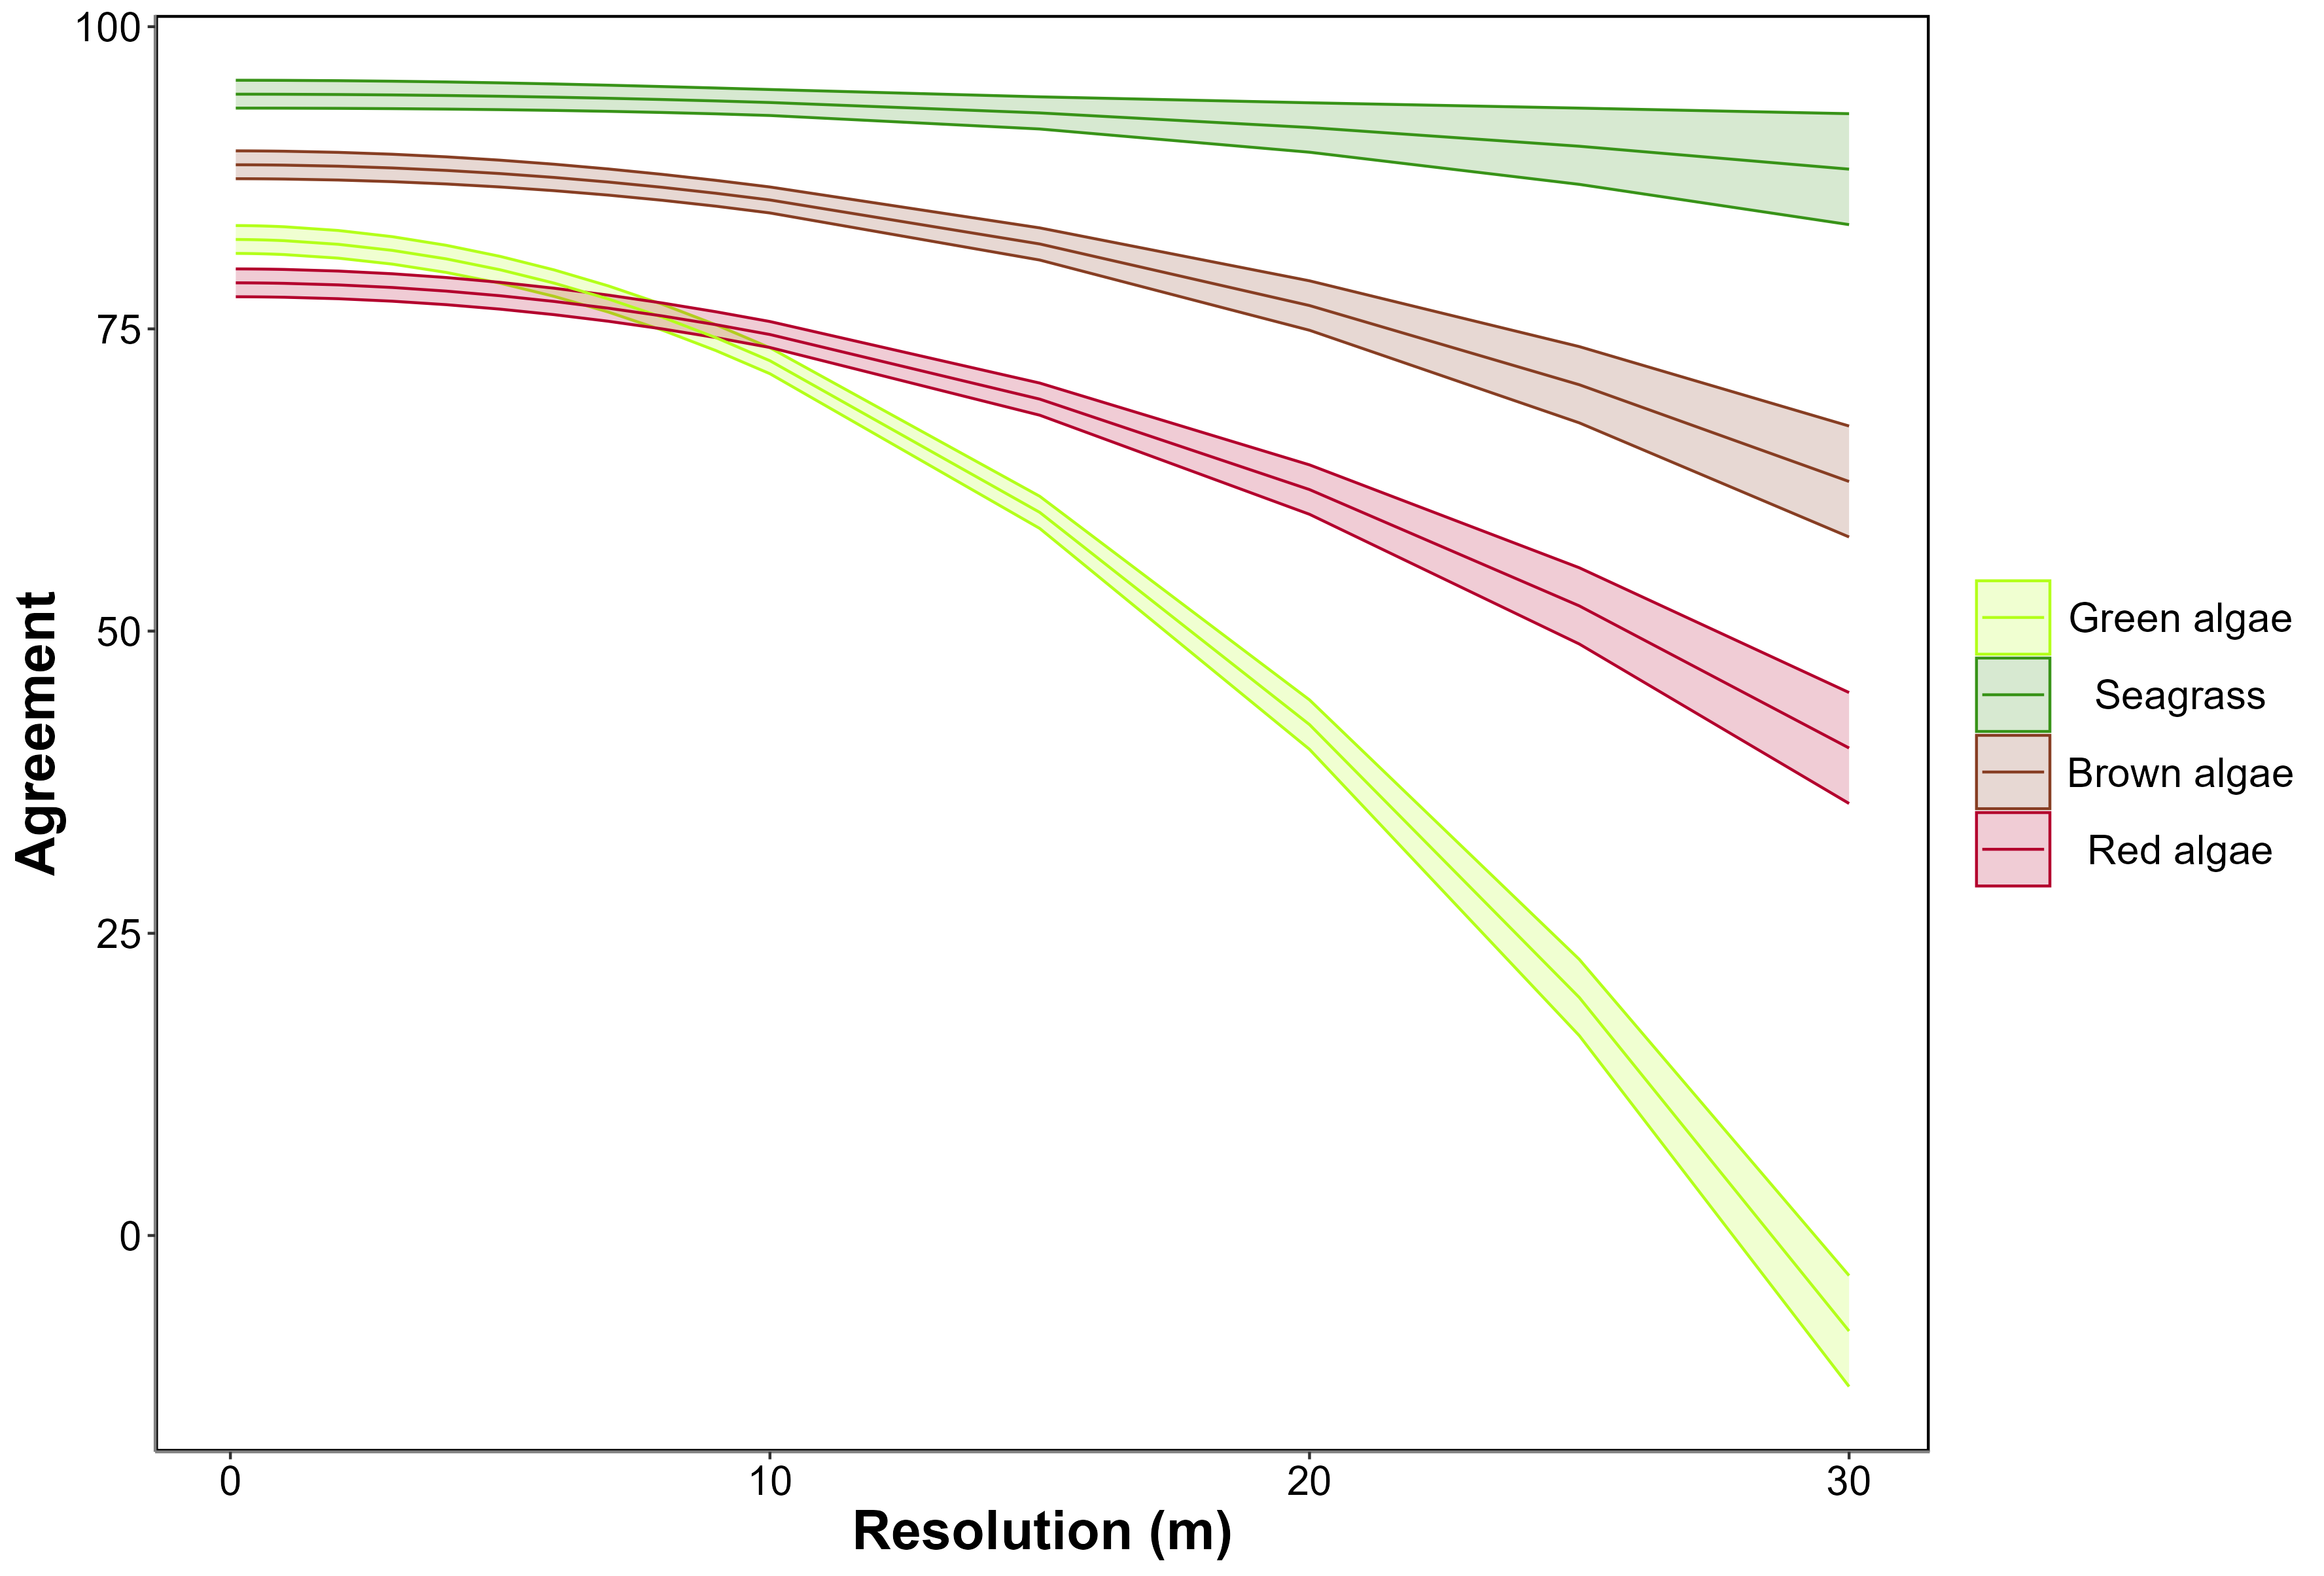
\includegraphics[width=0.9\textwidth,height=\textheight]{Figures/High_res/resolution_plot.png}

}

\caption{\label{fig-pixelsize}Coucou}

\end{figure}%

The Generalized Linear Model (GLM) analysis revealed a significant
effect of pixel resolution on the agreement, with a negative
relationship (\[\beta = -1.0334 \times 10^{-8}, p < 0.001\]). This
indicates that as pixel resolution increases, the proportion of the
response variable decreases.

The vegetation classes also exhibited distinct effects on the agreement.
Magnoliopsida showed a significant positive effect
(\[\beta = 0.1202, p < 0.001\]), suggesting that this class was
associated with a higher agreement.

\subsection{Effect of the percent cover on the
prediction}\label{effect-of-the-percent-cover-on-the-prediction}

Using the very high resolution low altitude flight (8 mm pixels), we
determined the minimal percent cover required to correctly classify a
given class within the corresponding high altitude flight
(Figure~\ref{fig-upscaling}).

\phantomsection\label{cell-fig-upscaling}
\begin{figure}[H]

\centering{

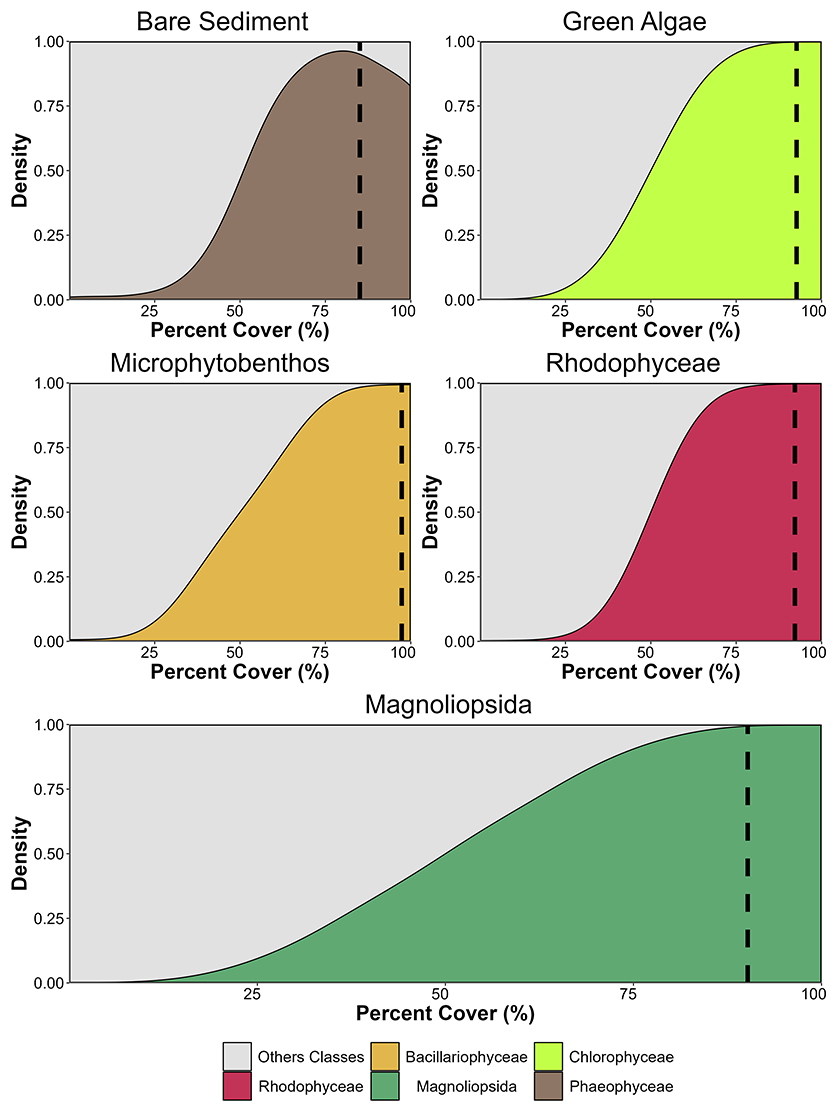
\includegraphics[width=0.9\textwidth,height=\textheight]{Figures/Low_res/Upscaling/density_vs_Proportion.png}

}

\caption{\label{fig-upscaling}Kernel density plot showing the proportion
of pixel well classified based on the percent cover of the class in high
altitude flight pixels of Gafanha, Portugal. Each subplot shows all the
pixels of the same classes on the high altitude flight. Percent cover of
classes was retrieved using the result of the classification of the low
altitude flight of Gafanha, Portugal.}

\end{figure}%

When the vegetation cover of a given class was 100 \%, coarser
high-flight pixels were well classified for all the classes except for
Bare Sediment, which was only well classified 80\% of the time. This
phenomenon may be attributed to the time gap between the two flights,
allowing for microphytobenthos migration to the surface during low tide,
consequently altering the model's classification from bare sediment to
Bacillariophyceae. A percent cover of at least 80\% was sufficient to
have all the pixels of high altitude flights correctly classified, with
the exception of Magnoliopsida that required a higher cover
(\textgreater90 \%) to be well classified. Concerning the probability of
each class, the highest percent cover was needed to confidently predict
Bacillariophyceae. To predict Chlorophyceae with a model likelihood of
0.85, a cover of 93 \% was needed, 90 \% for Magnoliopsida, 92 \% for
Rhodophyceae and 97 \% for Bacillariophyceae.

\section{Discussion}\label{discussion}

\subsection{Vegetation Discrimination}\label{vegetation-discrimination}

The primary objective of this study was to develop a method for the
accurate classification of macrophytes on intertidal mudflats and
sandflats, specifically focusing on distinguishing between Chlorophyceae
(green macroalgae) and marine Magnoliopsida (seagrasses) using
multispectral drone data. The ability to differentiate between various
types of vegetation plays a critical role in ecological monitoring and
coastal management \citep{WFD2000}. By distinguishing between seagrasses
and macroalgae, our approach facilitates targeted conservation
strategies, enabling more effective preservation and restoration efforts
in coastal ecosystems. The discrimination of seagrasses from green
macroalgae presents two main challenges \citetext{\citealp[
]{oiry2021using}; \citealp[
]{bannari2022}; \citealp{veettil2020opportunities}}. First these two
macrophytes have a similar pigment composition: chlorophyll-a (common to
all vegetation types), chlorophyll-b (an additional photosynthetic
pigment), and accessory carotenoids such as zeaxanthin, lutein and
neoxanthin (Figure~\ref{fig-Pigm}). Second, seagrass and green
macroalgae frequently co-occur in intertidal areas, and can intermingle
within a remote sensing pixel if the spatial resolution is too low.
Here, the issue of intra-pixel mixing was resolved thanks to the very
high spatial resolution of the drone, and the risk of spectral confusion
was avoided thanks to the efficiency of the multispectral classifier.
Our results confirm a recent study based on \emph{in situ} radiometry,
where it was demonstrated that a sensor with at least eight spectral
bands ranging from 500 to 850 nm and including a green band at 530 nm
and a RedEdge band at 730 nm was crucial to accurately discriminate
green macroalgae from seagrasses \citep{Davies2023}.

\phantomsection\label{cell-fig-Pigm}
\begin{figure}[H]

\centering{

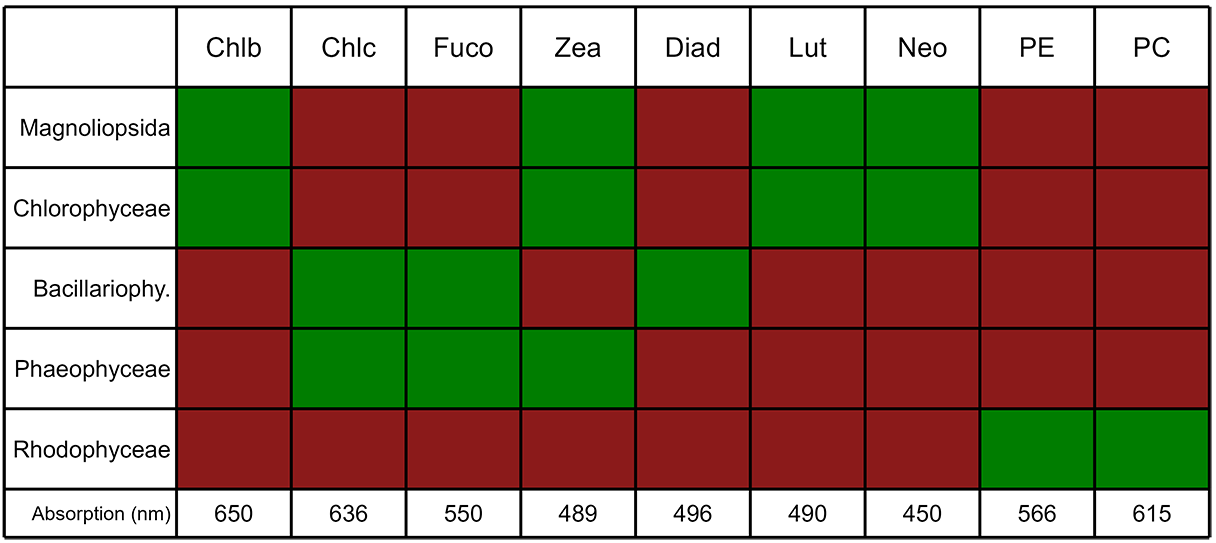
\includegraphics[width=1\textwidth,height=\textheight]{./Figures/Low_res/Disc_Pigment_Table.png}

}

\caption{\label{fig-Pigm}Photosynthetic and carotenoid pigments present
(Green) or absent (Red) in each taxonomic class present in the Neural
Network Classifier, along with their absorption wavelength measured with
spectroradiometer. Chl-b: chlorophyll-b, Chl-c: chlorophyll-c, Fuco:
fucoxanthin, Zea: zeaxanthin, Diad: diadinoxanthin, Lut: lutein, Neo:
neoxanthin, PE: phycoerythrin, PC: phycocyanin.}

\end{figure}%

\phantomsection\label{cell-fig-ValidationGreen}
\begin{figure}[H]

\centering{

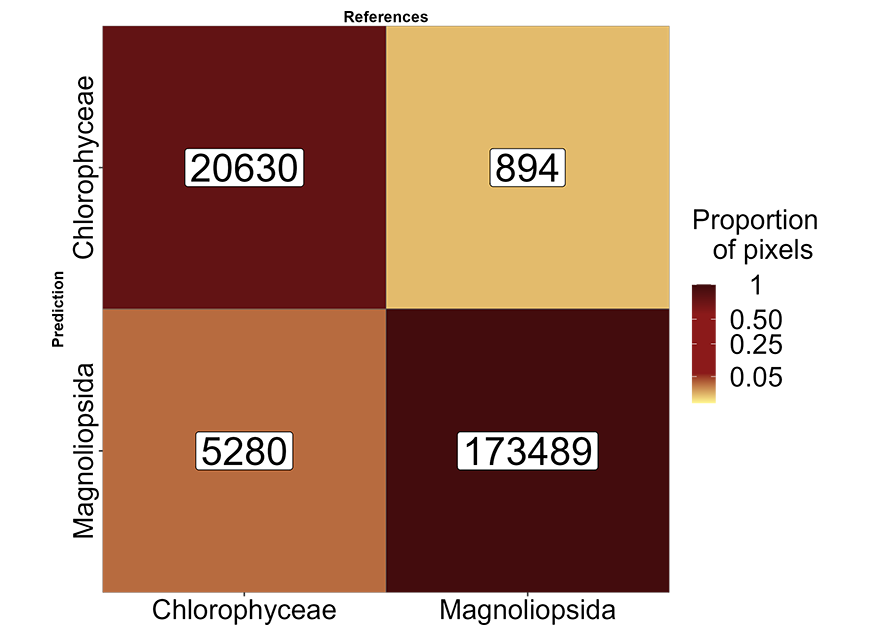
\includegraphics[width=1\textwidth,height=\textheight]{./Figures/Low_res/Validation/ConfusionMatrixGreen.png}

}

\caption{\label{fig-ValidationGreen}Sample of
Figure~\ref{fig-Validation} focusing on green macrophytes. The labels
inside the matrix indicate the number of pixels.}

\end{figure}%

Meeting these two criteria, the Micasense RedEdge-MX DUAL camera used in
this study, enabled the classifier to achieve 97\% of accuracy between
these two classes (Figure~\ref{fig-ValidationGreen}). Even if the
pigment composition of green macrophytes is similar, differences in the
spectral shape can be observed, with green algae having a higher
reflectance peak at 560 nm as well as a higher NIR plateau than seagrass
(Figure~\ref{fig-vegetation}). Such differences were previously
attributed to differences in pigments concentration and/or ratios
\citep{bargain2013seasonal}, cellular structure as well as in the
orientation of the plant over the sediment surface \citetext{\citealp[
]{beach1997vivo}; \citealp[
]{kirk1994light}; \citealp{hedley2018influence}}.

The variable importance analysis (Figure~\ref{fig-VIP}) identified that
the band at 531 nm was the most important for accurately identifying
Chlorophyceae. In fact, at this wavelength, Chlorophyceae exhibited the
highest reflectance among all other classes, highlighting the difference
in carotenoids to chlorophyll-a ratios between seagrasses and green
macroalgae \citep{repolho2017seagrass}.

Concerning Phaeophyceae, the thick cell walls of these macroalgae
\citep{charrier2021growth} make it more reflective in the infrared part
of the spectra \citep{Slaton2001} whereas the presence of fucoxanthin
and zeaxanthin result in a low reflectance in the visible region
(Figure~\ref{fig-Pigm} ; Figure~\ref{fig-VIP}). These two key features
have been identified by the Neural Network as the two principal
predictors to accurately identify brown algae (Figure~\ref{fig-VIP}).
Similarly, the presence of phycoerythrin and phycocyanin in Rhodophyceae
contribute to the lowest reflectance among all classes in the spectral
range from 560 to 615 nm (Figure~\ref{fig-VIP}). Indeed the band at 560
nm has been identified as important for identifying this class, likely
due to phycoerythrin absorption at this wavelength. Regarding
Bacillariophyceae, the VIP analysis (Figure~\ref{fig-VIP}) indicated
that 475 nm was the most important predictor for this class. Indeed, the
reflectance at 475 nm was higher for Bacillariophyceae than for any
other vegetation class (Figure~\ref{fig-vegetation}), very likely due to
the low biomass (and associated concentration of blue-absorbing
pigments) of microphytobenthos biofilms compared to seagrass and
macroalgae.

\subsection{Altitude and Temporal Effects on Vegetation Prediction
Accuracy}\label{altitude-and-temporal-effects-on-vegetation-prediction-accuracy}

While comparing the reflectance of both altitudes (12 m and 120 m), it
was observed that there is an underestimation of the infrared part of
the spectra in the high-altitude dataset (Figure~\ref{fig-CompareRef}).
Such disparity in infrared reflectance may stem from temporal
differences between the flights, possibly resulting in a slightly drier
intertidal area and consequently higher infrared reflectance. This
disparity poses an issue for the methodology followed in the present
study, relying solely on one flight height for training. To address this
issue, we employed min/max standardized reflectance spectra as
predictors for the model Equation~\ref{eq-std}. This approach allowed us
to eliminate the slight reflectance difference between the flights
(Figure~\ref{fig-CompareRef} B) and to focus on the shape of the spectra
in the visible part of the electromagnetic spectra, where different
pigmentation are associated to taxonomic dignostic features. This was a
key feature in building a model that could reliably predict vegetation
across geographical sites and seasons. It enabled consistent prediction
of vegetation classes across variations in biomass and variability in
light conditions \citetext{\citealp[ ]{fyfe2003spatial}; \citealp[
]{COSTA2021107018}; \citealp{piaser2023impact}}.

We found 90 \% of seagrass cover is necessary for confident prediction
of its presence (Figure~\ref{fig-upscaling}). This highlights a
limitation of the methodology used to construct the training dataset for
the model. The dataset used to train our algorithm was composed
exclusively of pure pixels, which resulted in the model's reduced
confidence when faced with lower percentages of seagrass cover. Also,
intertidal seagrasses exhibit marked phenology, with varying pigment
composition throughout the year \citetext{\citealp[
]{bargain2013seasonal}; \citealp{legare2022remote}}. Since the training
dataset has been made using well established seagrass meadows, this
model may be less accurate outside of the seasonal seagrass peak of
biomass. Further investigation is required to evaluate the accuracy of
the method along different periods of the year.

\subsection{Towards climate and biodiversity
applications}\label{towards-climate-and-biodiversity-applications}

Climate change, global warming, eutrophication, alien and invasive
species development, coastal erosion, and sealevel rise are expected to
continue impacting coastal ecosystems in the future
\citetext{\citealp{SCHIBALSKI2022101414}; \citealp[
]{holon2018predictive}; \citealp{marquet2024global}}. and the demand for
meaningful and efficient monitoring of coastal habitats has never been
higher\citetext{\citealp[ ]{muller2018satellite}; \citealp[
]{villalobos2023remote}; \citealp{oiry2021using}}. Our findings,
particularly the improved discrimination of intertidal seagrass and
green macroalgae from other intertidal vegetation classes, highlight the
potential of drone-based remote sensing to support diverse applications,
from conservation of biodiversity to climate change adaptation
strategies.

Because of coastal eutrophication, macroalgal blooms are becoming
increasingly common in many regions around the world \citetext{\citealp[
]{sutton2011european}; \citealp{ye2011green}}. These blooms can have
negative impacts on human health and local economic activities,
including human health, fishing and aquaculture, tourism, and
recreational activities \citetext{\citealp[
]{villares1999nitrogen}; \citealp{ye2011green}}. The first green tide
events (i.e.~bloom of green macroalgae of the genus \emph{Ulva}) were
reported in Brittany, France, back in the 1970s and have since been a
concern for local stakeholders and economic activities
\citep{menesguen2018marees}. Some regions of the world have witnessed an
increase in brown macroalgae blooms, predominantly involving algae of
the genus \emph{Sargassum} washing along the Caribbean coastlines
\citep{louime2017sargassum}, and more recently \emph{Rugulopteryx
okamurea} in southern Europe \citep{Roca2022}. Satellite remote sensing
has proven to be a valuable tool for mapping the spatial and temporal
extent of macroalgal blooms worldwide. However, due to limitations in
spatial resolution, it can only effectively map well-developed blooms
\citetext{\citealp[ ]{rs13081408}; \citealp[
]{klemas2012remote}; \citealp{haro2023biointertidal}}. High spatial
resolution drone imagery, coupled with an accurate classification
algorithm, could be used to map the early stages of macroalgal blooms in
areas known to have regular blooms or in new sites. Indeed, this
approach could provide early warning alerts to local managers.

Employing traditional sampling methods to monitor coastal ecosystems is
time and resource-intensive, and the findings are often difficult to
scale-up. Earth Observation can bridge this gap and meet the needs for
systematic monitoring coastal ecosystems over large areas
\citep{papathanasopoulou2019satellite}. The retrieval of Essential
Biodiversity Variables and Essential Ocean Variables through satellite
observations has been increasingly common, enabling comprehensive
monitoring of entire ecosystems over extended time periods
\citetext{\citealp[ ]{ratnarajah2023monitoring}; \citealp{Zoffoli2021}}.
The Water Framework Directive \citep{WFD2000} mandates the achievement
and maintenance of ``good ecological status'' for all European waters,
which necessitates a comprehensive understanding and monitoring of
aquatic ecosystems, including coastal habitats like seagrass beds
\citetext{\citealp[ ]{foden2007angiosperms}; \citealp[
]{nordlund2024one}; \citealp{Zoffoli2021}}.

Effective and efficient monitoring tools are essential for identifying
the impacts of human activities and natural changes on coastal
ecosystems. On-demand, multispectral drone observations at very high
spatial-resolution provide a novel and powerful tool to rapidly and
accurately acquire ground truth satellite data. Spatially resolved data
are indeed critical for calibrating and validating satellite remote
sensing observations, thereby enhancing our capacity to monitor vast
coastal areas. A perspective of this work could be to develop a similar
classifier for satellite images (e.g.~Sentinel-2), and test whether the
discrimination between seagrass and green macroalgae is still
operational at a coarser spatial resolution. The integration of drone
technology facilitates a scalable approach to environmental
surveillance, offering significant advancements in the spatial and
temporal resolution of data collection. This, in turn, supports the EU
WFD's objectives by enabling more informed and timely management
decisions for the conservation and restoration of aquatic ecosystems.

\section{Conclusion}\label{conclusion}

The utilization of very high spatial-resolution drone-based remote
sensing coupled with machine learning techniques has proven to be an
effective method for the discrimination of intertidal seagrasses from
green macroalgae with a multispectral resolution sensor. Standardized
reflectance was incorporated in the Neural Network model allowing for a
better discrimination of spectral features related to pigment absorption
in the visible region of the spectrum. There was a striking difference
for the variable of importance to discriminate Magnoliopsida from
Chlorophyceae. The latter was essentially identified with the 451 nm
spectral band while more spectral bands were needed to identify the
former, notably 650, 560, 668, and 705 nm. As the spectral bands of the
Micasense RedEdge Dual MX are very similar to those of Sentinel-2, we
suggest that multispectral satellite data have the potential to perform
this discrimination between green these macrophytes. A Sentinel-2
algorithm could be developed, using the output of this current workflow
as training and validation data. The findings underscore the importance
of adopting advanced remote sensing tools in ecological studies and
environmental monitoring, providing a foundation for future research and
policy implementation aimed at ecosystem conservation and restoration.


  \bibliography{library.bib}


\end{document}
